\renewcommand{\typeRubriek}{loep}		

% twee parameters voor nieuwe rubriek: titel en auteur (die mogen ook leeggelaten worden o.a. voor redactioneel)
\startNieuweRubriek{{\doublespacing Lineair\\ programmeren}}{Johan Deprez\\ Michel Roelens}
\vspace{1.5cm}

\startcontents[mainsections]		% opsomming in inhoudstafel enkel tot loep beperken


% tekst van de loep %
%%%%%%%%%%%%%%%%%%%%%

\begin{multicols}{2}
	
	\inhoudstafelLoep		            % inhoudstafel invoegen, verder niets mee doen
	
	%Timing
	

	
\section{Inleiding}
	
    Lange tijd hadden economische studierichtingen in het secundair onderwijs slechts een beperkt pakket aan wiskunde. Later ontstond een tweedeling: er kwam een studierichting economie-wiskunde, met een stevig pakket aan wiskunde, naast economische studierichtingen waarvoor het pakket aan wiskunde beperkt bleef. Na de recente herziening van de eindtermen in de derde graad, die over enkele jaren geïmplementeerd wordt, zal deze tweedeling blijven bestaan (economie-wiskunde versus andere economische studierichtingen), maar wordt het pakket aan wiskunde in deze andere economische studierichtingen toch wat verstevigd. Bovenop de basiseindtermen krijgen de leerlingen uit de doorstroom studierichtingen economie-moderne talen en de nieuwe studierichting bedrijfswetenschappen binnenkort ook een set specifieke eindtermen ‘uitgebreide wiskunde in functie van economie’ (AHOVOKS, s.d.). Dat is een goede zaak: in vervolgopleidingen krijgen deze leerlingen immers vaak heel wat wiskunde en statistiek.
	
    Een van de nieuwe specifieke eindtermen (nummer 6.3.9) luidt als volgt: “De leerlingen lossen optimalisatieproblemen op met behulp van lineaire programmering.” In het secundair onderwijs is lineaire programmering niet helemaal nieuw: het is bijvoorbeeld een keuzeonderwerp in de huidige leerplannen voor sommige kso- en tso-richtingen. In economische opleidingen in het hoger onderwijs is het een klassieker. Het is bijvoorbeeld een onderdeel van operationeel onderzoek, typische wiskunde van de handelsingenieur. We hebben er in Uitwiskeling al eens eerder een loep aan besteed (Kesselaers, Kesteloot en Roels, 1986).
    
    Een interessant aspect van lineaire programmering is de combinatie van het visuele (het werken op de grafiek) en het algebraïsche. Wat je doet met de ongelijkheden en de winst- of kostenfunctie, of wat je in de matrices doet bij de simplexmethode, kun je grafisch interpreteren en de inspiratie voor wat je algebraïsch doet komt van het grafische. Dat over en weer gaan leidt tot inzicht. Bovendien geeft het een inkijk in enkele echte toepassingen van ongelijkheden. 
    
    Je zult zien dat deze combinatie van het visuele en het algebraïsche de rode draad vormt doorheen deze loep. Daarmee gaan we verder dan wat in de eindterm gevraagd wordt: het gebruik van matrices en de simplexmethode is niet in de eindterm opgenomen. Ook bij het grafisch oplossen voorzien we enkele uitbreidingsoefeningen, waarin gebruik gemaakt wordt van parameters.

    De meeste opgaven hebben we niet zelf verzonnen. Voor zover we ze terugvinden, proberen we wel de oorspronkelijke bron te vermelden. Het is goed om bij de eerste opgaven op papier te werken. Na een tijd kunnen leerlingen gerust gebruik maken van GeoGebra, de grafische rekenmachine, Excel of een online-app. In 2.3 vertellen we iets meer over deze digitale hulpmiddelen. Dat wil niet noodzakelijk zeggen dat alle opgaven die daarvoor staan, met de hand moeten worden opgelost.


\section{ Grafische methode met twee variabelen}
	
\subsection{De winst maximaliseren}

    Bij lineaire programmering zoeken we steeds naar een maximale winst of een minimale kost binnen bepaalde randvoorwaarden. We starten met het maximaliseren van winst. Hieronder brengen we grafische methodes aan:  de \emph{schuifmethode} en de \emph{hoekpuntenmethode}. In paragraaf 3 zullen nog andere methoden aan bod komen: de \emph{wandelmethode} en de (algebraïsche) \emph{simplexmethode}. We besteden bij het eerste voorbeeld veel aandacht aan de verschillende stappen bij het maken van de tekening: het tekenen van de oplossingen van een eerstegraadsvergelijking en een eerstegraadsongelijkheid, de isolijnen (in dit geval: rechten van gelijke winst) en het grafisch bepalen van de oplossing van het probleem. Indien nodig kun je de leerlingen vooraf laten oefenen op het grafisch oplossen van eerstegraadsvergelijkingen, stelsels, ongelijkheden.

    De eerste werktekst is geïnspireerd door Math4all (s.d.).

\end{multicols}

\beginwerktekst{Fietsen en e-bikes}

    \begin{kader}
    	De verkoop van fietsen en e-bikes zit in de lift.
    	
	    Een fietsenhandelaar krijgt van de fabrikant een aanbod van fietsen en e-bikes tegen een inkoopprijs van $\euro 500,00$ per fiets en $\euro 900,00$ per e-bike. 
	
	    De handelaar wil maximaal $100$ fietsen en $200$ e-bikes bestellen. Hij beschikt hiervoor over een totaal budget van $\euro 190\, 000,00$. Verder heeft hij maar $120\; \mathrm{m}^2$ opslagruimte voor deze bestelling, waarbij hij voor een fiets en een e-bike $0,5\;\mathrm{m}^2$ per stuk rekent.
	
	    Per fiets kan hij € 200,00 winst maken en per e-bike € 300,00.
	
	    Hoeveel winst kan hij maximaal maken op dit aanbod?
    \end{kader}

    \begin{werktekstoef}
    

	\item Waarom kan hij niet gewoon 100 fietsen en 200 e-bikes verkopen, en bijgevolg $100\cdot 200 + 200\cdot 300 = 80\,000$ euro winst maken?
	
	\emph{Dat zou hem $\euro 230\,000$ kosten; dit overschrijdt zijn budget. Bovendien zou hij daarvoor $150\; \mathrm{m}^2$ opslagruimte nodig hebben. Hij wil zoveel mogelijk winst maken, maar wel rekening houdend met de randvoorwaarden van het beschikbare budget en de opslagruimte.}
	
	\item Het is een probleem met twee variabelen waarvan de handelaar, binnen bepaalde beperkingen, zelf de waarden kan kiezen. Daarom spreekt men van \emph{beslissingsvariabelen}. Meestal worden die variabelen in de wiskunde $x$ en $y$ genoemd. Wat zijn in dit probleem $x$ en $y$?
	
	\emph{$x =$ het aantal fietsen dat hij bestelt; $y=$ het aantal e-bikes dat hij bestelt. Merk op: ``$x=$ aantal fietsen'' is ook goed maar ``$x=$ fietsen'' wordt niet goed gerekend.}
	
	\item De randvoorwaarden zijn: het aantal fietsen moet tussen 0 en 100 liggen, het aantal e-bikes tussen 0 en 200, en dan zijn er de randvoorwaarden door het beschikbare budget en de opslagruimte. Druk de randvoorwaarden uit met $x$ en $y$. Vereenvoudig als dat mogelijk is.
	
	\emph{Dit geeft:}
	
	$$
	\left\{
	\begin{array}{ccr}
		
		0\;\; \le \;\;\;\;\;\;\;\; x &\le &100 \\
		0\;\;\le \;\;\;\;\;\;\;\; y &\le &200 \\
		500x+900y &\le  &190\,000 \\
		0,5x+0,5y &\le  &120
		
	\end{array}
	\right.
	$$
	
	\emph{Of vereenvoudigd:}
	
    $$
    \left\{
    \begin{array}{ccr}
    	
    	0\;\; \le \;\;\;\;\;\;\;\; x &\le &100 \\
    	0\;\;\le \;\;\;\;\;\;\;\; y &\le &200 \\
    	5x+9y &\le  &1900 \\
    	x+y &\le  &240
    	
    \end{array}
    \right.
    $$  

    \item Druk ook de winst (als alles verkocht wordt) uit in $x$ en $y$. 
    
    \emph{Antwoord: $\mathrm{winst} = 200 x+ 300 y$.}
    
    \end{werktekstoef}
    
    Deze winstfunctie in twee variabelen is een voorbeeld van een \emph{doelfunctie}. Er is bij lineaire programmering altijd een doelfunctie die je moet minimaliseren of maximaliseren. In dit geval is de doelfunctie een winstfunctie, maar soms is het een kostenfunctie en die wil je natuurlijk klein houden... 
    
    \begin{werktekstoef}
    
    \setcounter{enumi}{4}
        
    \item Eén van de randvoorwaarden is, na vereenvoudiging, $5x+9y\le 1900$. Dit is de beperktheid van het budget. Om de oplossingen van deze ongelijkheid in een assenstelsel te tekenen, teken je eerst de rechte $5x+9y=1900$. De oplossingenverzameling van de \emph{on}gelijkheid is één van de halfvlakken bepaald door deze rechte. Aan één kant van die rechte (binnen het kwadrant waar $x$ en $y$ positief zijn) heb je bestellingen die binnen het budget vallen en aan de andere kant van die rechte bestellingen die het budget overschrijden. Teken het juiste halfvlak en leg uit hoe je het vindt.
	
	\emph{Om de rechte te tekenen, kunnen de leerlingen twee punten van de rechte tekenen en verbinden. Het gemakkelijkste is hier de snijpunten met de assen te zoeken. Het snijpunt met de $x$-as vinden ze door $y$ gelijk aan nul te stellen: $(380, 0)$. Het snijpunt met de $y$-as vinden ze door $x$ gelijk aan nul te nemen: $(0, \frac{1900}{9})\approx(0; 211,11)$. Om de `juiste kant' van die rechte te bepalen, kunnen leerlingen een gemakkelijke oplossing van de ongelijkheid nemen, bv. $(0, 0)$. Niets bestellen valt zeker binnen het budget... Het halfvlak waar deze oplossing in ligt, is dan de wiskundige oplossingenverzameling van de ongelijkheid. De bestellingen die binnen het budget vallen, liggen in de driehoek die de doorsnede is van dit halfvlak met het eerste kwadrant.}

	\begin{center}
	\includegraphics[width=0.6\linewidth]{img/linprog1}
    \end{center}
	
	\item Er zijn nog andere randvoorwaarden. De punten $(x, y)$ die aan \emph{alle} randvoorwaarden voldoen, vormen het \emph{toegelaten gebied} (of: \emph{toegestane} gebied) van dit probleem. Teken dit gebied.
	
	\emph{De leerlingen vinden het gearceerde gebied $OABCDE$, als doorsnede van de oplossingenverzamelingen van de aparte ongelijkheden.}
	
	\begin{center}
	    \includegraphics[width=0.6\linewidth]{img/linprog2}
	\end{center}
	
	\end{werktekstoef}
	
	Nu willen we op zoek naar het punt met maximale winst. Om dat te doen, kijken we eerst waar de punten liggen met een welbepaalde winstwaarde.
	
	\begin{werktekstoef}
	
	\setcounter{enumi}{6}
	
	\item Waar liggen alle punten $(x, y)$ waarbij de winst gelijk is aan $\euro 20\,000$? Duid die aan op de tekening.
	
	\emph{Deze punten voldoen aan de vergelijking $200x+300y=20\,000$ (of vereenvoudigd $2x+3y=200$). Ze vormen dus een rechte. (Zie figuur onder de volgende vraag.)}
	
	\item En waar liggen de punten $(x, y)$ waarbij de winst gelijk is aan $\euro 40\,000$? En aan 60 000 euro? En aan 80 000 euro?
	
	\emph{Op de rechten $2x+3y=400$, $2x+3y=600$ respectievelijk $2x+3y=800$. (Zie figuur.) Merk op dat deze laatste rechte volledig buiten het toegelaten gebied valt. Een winst van 80 000 euro is dus, binnen de vooropgestelde beperkingen, niet mogelijk.}
	
	\begin{center}
	    \includegraphics[width=0.6\linewidth]{img/linprog3}
	\end{center}
	
	\end{werktekstoef}
	
	Een rechte van gelijke winst is een voorbeeld van een \emph{isolijn}. `Iso' komt van het Griekse $\iota\sigma o\varsigma$, gelijk. In aardrijkskunde ontmoet je isobaren, isothermen, enz. (lijnen van gelijke luchtdruk, temperatuur...). Deze lijnen zijn niet recht. Bij `lineaire programmering', waar het in deze loep over gaat, zijn de iso-winstlijnen en de iso-kostenlijnen wel rechten, net als de randen van het toegelaten gebied, vandaar `lineaire' in de naam lineaire programmering.
	
    \begin{werktekstoef}
    
    \setcounter{enumi}{8}

    \item Vergelijk de getekende rechten van gelijke winst. Wat stel je vast?
    
    \emph{Ze zijn evenwijdig. Hoe verder van de oorsprong, hoe groter de winst.}
    
    \end{werktekstoef}
    
    Als de winst geleidelijk groter wordt, verschuift de rechte van gelijke winst geleidelijk weg van de oorsprong. Dit geeft een manier om het punt van het toegelaten gebied te vinden waar de winst maximaal is: de \emph{schuifmethode}.
    
    \begin{werktekstoef}
    
    \setcounter{enumi}{9}
    
    \item In welk punt van het toegelaten gebied is de winst maximaal? Leg uit.
	
	\emph{In het punt $C$. Immers, als de rechte van gelijke winst geleidelijk naar rechtsboven verschuift, wordt de winst groter. Het laatste punt van het toegelaten gebied dat deze rechte ontmoet, is punt $C$.}
	
	\item Hoeveel fietsen en hoeveel e-bikes moet de fietsenhandelaar nu bestellen? En hoeveel winst maakt hij als hij die allemaal verkoopt?
	
	\emph{Het aantal fietsen en e-bikes zijn de $x$- en de $y$-coördinaat van het punt $C$. Je vindt die door het stelsel}
	
    $$
    \left\{
    \begin{array}{ccl}
    	
    	5x+9y &= &1900 \\
    	x+y &= &240
    	
    \end{array}
    \right.
    $$
    
	\emph{op te lossen. De oplossing is: $x=65; y=175$. De fietsenhandelaar moet $65$ fietsen en $175$ e-bikes bestellen om zoveel mogelijk winst te kunnen maken.}
	
	\item Hoeveel winst maakt de fietsenhandelaar als hij alles verkocht krijgt?
	
	\emph{We vullen de oplossing $(65, 175)$ in in de winstfunctie. Dit geeft: $\mathrm{winst}= 200\cdot 65+300\cdot 175=65\,500 $. De fietsenhandelaar kan dus $\euro 65\,500$ winst maken.}
	
	\end{werktekstoef}
	
    Door de redenering van de schuifmethode weten we dat er altijd een hoekpunt zal zijn waar de winst maximaal is. 
    
    Een andere methode in plaats van de schuifmethode is de \emph{hoekpuntenmethode}: bereken de winst in elk hoekpunt van het toegelaten gebied en kijk waar de winst het grootste is.
	
	\begin{werktekstoef}
	
	\setcounter{enumi}{12}
	    
	\item Noem van beide methoden een voordeel.
	
	\emph{Voordeel van de schuifmethode: je moet de winst maar in één hoekpunt berekenen. Voordeel van de hoekpuntenmethode: je hoeft geen rechten van gelijke winst te tekenen.}
	
	\item Pas de hoekpuntenmethode even toe om de(zelfde) oplossing van dit fietsenprobleem te vinden. Ben je klaar, dan mag je gaan fietsen.
	
	\emph{De leerlingen bepalen de coördinaten van de hoekpunten en vullen die in in de winstfunctie. Ze stellen vast dat de grootste winst inderdaad bereikt wordt in punt $C$.}

    \end{werktekstoef}
    
\eindewerktekst
    
\begin{multicols}{2}
        
    Na deze opdracht (en ook bij andere opdrachten) is het goed om de leerlingen aan te moedigen om kritiek te formuleren op de opgave. Bv. hoe realistisch is het dat de fietsenwinkel maar twee soorten fietsen verkoopt? Is $0,5\;\mathrm{m}^2$ voldoende om een e-bike te stockeren? Komt het altijd mooi uit op gehele waarden voor de twee variabelen? Als we $x=65,5$ waren uitgekomen, hadden we dan een fiets in twee moeten zagen? (Zie paragraaf 2.4 in verband met niet-gehele oplossingen.)
    
    Je kunt ook, nu of na nog enkele oefeningen, aan een leerling vragen om de oplossingsmethode in het algemeen, zonder verwijzing naar fietsen en zonder concrete getallen, uit te leggen. Wat doe je eerst? En dan? Hierbij worden de begrippen randvoorwaarden, toegelaten gebied, doelfunctie, isolijnen (hier: rechten van gelijke winst), schuifmethode, hoekpuntenmethode op het bord bij elkaar gezet.
    
    Voor leerlingen met masterplannen is het zeker ook nodig om de terminologie in het Engels te vermelden:
    
    \begin{center}
        
    \begin{tabular} {|l|l|}
        \hline
         randvoorwaarden & \emph{constraints}\\
         beslissingsvariabelen & \emph{decision variables}\\
         toegelaten gebied &  \emph{feasable region}\\
         doelfunctie & \emph{objective function}\\
         winst & \emph{profit}\\ 
         kosten & \emph{cost}\\ 
         isolijnen  & \emph{contour lines }\\
         lijnen van gelijke winst & \emph{iso-profit lines}\\
        \hline
    \end{tabular}
    
    \end{center}
    
    We geven nog twee oefeningen, een `kaal' probleem en een probleem over tennisrackets. Dat laatste vonden we in math4all.

\end{multicols}

\beginwerktekst{Nu helemaal zelf}

	\begin{werktekstoef}
	
	\item Los dit lineaire programmeringsprobleem op met de schuifmethode. 
	
    $$
    \left\{
    \begin{array}{rrcl}
    	
          &\;\;\;\;0\;\;\;\;\le \;\;\;\;x &\le &10 \\
          &\;\;\;\;0\;\;\;\;\le \;\;\;\;y &\le & 8 \\
    	  &x+2y &\le  &18 \\
    	  &x+y &\le  &13 \\
    	  &200x+300y&=&\mathrm{winst}
    	
    \end{array}
    \right.
    $$  

    \emph{De oplossing is $x= 8 ; y= 5 $. De maximale winst is $3100$ (munteenheden; er staat niet bij of het euro is). Zie figuur.}
	
	\begin{center}
	    \includegraphics[width=0.6\linewidth]{img/linprog4}
	\end{center}
	
	\item In een fabriek worden twee soorten tennisrackets gemaakt, rackets met een aluminium frame en rackets met een kunststof frame. De winst op een racket met een aluminium frame is $\euro 55,00$, voor een racket met een kunststof frame is dat $\euro20,00$. 
	
	De rackets worden deels machinaal gemaakt, maar er is ook handenarbeid voor nodig: de machines moeten bediend worden.
	
	Het machinepark van het bedrijf kan per dag 30 aluminium rackets maken, of 150 kunststof rackets, of een combinatie hiervan (bv. 15 aluminium rackets en 75 kunststof rackets, of 10 aluminium rackets en 100 kunststof rackets of...). Het komt er eigenlijk op neer dat voor een aluminium racket het machinepark $\frac{1}{30}$ van een dag moeten draaien en voor een kunststof racket $\frac{1}{150}$ van een dag.
	
	Er werken 20 mensen aan de productie van deze rackets. Voor het maken van twee aluminium rackets is één persoon een hele dag bezig, terwijl één persoon per dag vijf kunststof rackets kan produceren.
	
    De bedrijfsleidster wil zo veel mogelijk winst maken. 
    Schrijf dit als een stelsel van ongelijkheden en een winstfunctie. Los grafisch op en geef de bedrijfsleidster advies.
    
    \emph{Noem $x$ het aantal aluminium rackets en $y$ het aantal kunststof rackets dat per dag geproduceerd wordt. Naast $0\le x; 0\le y$: zijn er twee randvoorwaarden: het machinepark kan per dag maximaal de hele werkdag aan het draaien zijn, verdeeld over de twee soorten rackets, en er zijn per dag 20 mensen die maximaal de hele werkdag aan de productie besteden. De doelfunctie is de winst per dag.}

    $$
    \left\{
    \begin{array}{rcl}
        \,\,x &\ge &0\\
        \,\,y &\ge &0\\
        \, \frac{1}{30} x +  \frac{1}{150} y &\le  &1 \\
        \, \frac{1}{2}  x+\frac{1}{5} y &\le  &20 \\
        \, 55x+20y&=&\mathrm{winst}
    \end{array}
    \right.
    $$  

    \emph{Vereenvoudigen geeft:}

    $$
    \left\{
    \begin{array}{rcl}
        \,\,x &\ge &0\\
        \,\,y &\ge &0\\
    	5x+y &\le  &150 \\
    	\, 5x+2y&\le  &200 \\
    	\, 55x+20y&=&\mathrm{winst}
    \end{array}
    \right.
    $$
    
     \emph{De oplossing is $A(20,50)$, zie figuur. Merk op: de eenheden op de assen zijn niet even groot getekend. Ons advies is dus: maak per dag 20 rackets met aluminium frames en 50 met kunststof frames. Als je die allemaal verkoopt is de dagelijkse winst $\euro 2100$.}
	
	\begin{center}
	    \includegraphics[width=0.55\linewidth]{img/linprog5}
	\end{center}	

	\end{werktekstoef}
	
	\eindewerktekst
	
	
	\begin{multicols}{2}
	    
    \subsection{De kosten minimaliseren}

    Het grafisch oplossen van problemen waarbij je kosten moet minimaliseren, is analoog aan die waarbij je de winst moet maximaliseren. De volgende opgave is gebaseerd op Goemaere (2010).

    \end{multicols}

    \beginwerktekst{Gepakt en gezakt op schoolreis}

	\begin{kader}
	
    	Je school organiseert een reis van vijf dagen naar Bretagne. De reis gebeurt met huurbusjes. Er zijn twee soorten huurbusjes beschikbaar: Volkswagen en Ford. In totaal gaan 105 personen mee (leerlingen en leerkrachten) en 64 valiezen bagage. In een Volkswagen-busje kunnen 7 personen en 6 valiezen. In een Ford-busje kunnen 9 personen en 4 valiezen. De busjes kosten $\euro 60$ per dag voor een Volkswagen en $\euro 55$ voor een Ford. 
    	
    	Hoeveel busjes van elke soort moet de school huren om de reis zo goedkoop mogelijk te houden?
    	
    \end{kader}
	 \begin{center}
        
\includegraphics[width=0.75\linewidth]{img/UW 21 bus.jpg}
    \end{center}
    \begin{werktekstoef}
    
    \item Kies de beslissingsvariabelen en schrijf het probleem als een stelsel van randvoorwaarden en een doelfunctie. Wat is het verschil met de opgaven tot hier toe?
    
    \emph{Noem $x$ het aantal Volkswagenbusjes en $y$ het aantal Fordbusjes. Er is een randvoorwaarde voor de personen die mee moeten en een andere randvoorwaarde voor de bagage. Merk op dat de ongelijkheden nu omgekeerd zijn vergeleken met de vorige opgaven: er moeten \emph{minstens} zoveel mensen en zoveel valiezen mee. De doelfunctie is nu geen winst maar een kost en die moet minimaal zijn.}
    
    $$
    \left\{
    \begin{array}{rcl}
         x &\ge &0\\
         y &\ge &0\\
    	 7x+9y &\ge  &105 \\
    	 6x+4y&\ge  &64 \\
    	 60x+55y&=&\mathrm{kosten}
    \end{array}
    \right.
    $$ 
    
    \emph{De vierde ongelijkheid kunnen we vereenvoudigen. }
    
    $$
    \left\{
    \begin{array}{rcl}
         x &\ge &0\\
         y &\ge &0\\
    	 7x+9y &\ge  &105 \\
    	 \, 3x+2y&\ge  &32 \\
    	 \, 60x+55y&=&\mathrm{kosten}
    \end{array}
    \right.
    $$
    
    \emph{Merk op dat we de kostenfunctie niet mogen vereenvoudigen tot ``$12x+11y=\mathrm{kosten}$''; het rechterlid zou dan niet meer in euro uitgedrukt zijn maar in eenheden van $5$ euro. ``$12x+11y=\frac{1}{5}\cdot \mathrm{kosten}$'' zou wel juist zijn.}
    
    \item Teken het toegelaten gebied en bepaal de oplossing met de schuifmethode. Is het toegelaten gebied begrensd?
    
    \emph{Nu behoort $(0, 0)$ niet tot de oplossingenverzamelingen van de ongelijkheden. We moeten de andere kant nemen. Het toegelaten gebied is nu onbegrensd.}
    
    \begin{center}
        \includegraphics[width=0.45\linewidth]{img/linprog6}
    \end{center}
    	
    \emph{De kosten worden hoger naarmate de iso-kostenlijn weg van de oorsprong, naar rechtsboven, verschuift. De oplossing is dus het hoekpunt van het toegelaten gebied dat als eerste aangeraakt wordt door de iso-kostenlijn die vanuit de oorsprong naar rechtsboven schuift. Dit is het punt $(6,7)$. De goedkoopste oplossing is $6$ busjes van Volkswagen en $7$ busjes van Ford huren.}
    
    \end{werktekstoef}
\eindewerktekst
    
\begin{multicols}{2}
    
    Een andere context voor het minimaliseren van kosten, is het samenstellen van een dieet. De volgende oefening, over een heel eenvoudig dieet voor pony's, komt uit de Wageningse Methode (van den Broek e.a., 2008).
    
    \end{multicols}
    
    \beginwerktekst{Pony's voederen}
 
    Naomi wil haar pony's gezond voederen. In de winter krijgen ze `biks' (een soort geperste staafjes) en hooi. De belangrijkste bestanddelen van dit voer 
    zijn:
    
    \begin{opsomming}
    \item koolhydraten, die zorgen voor de energievoorziening, 
    \item eiwitten,  die  van  groot  belang  zijn  voor de vorming van 
    spieren, hoeven, bloed...   
    \end{opsomming}
    
    Whiskey, één van haar pony's, die soms een beetje zwalpt, heeft per dag $2100\; \mathrm{g}$ koolhydraten  en  $360 
    \; \mathrm{g}$ eiwitten nodig. In één kg biks zit $600\; \mathrm{g}$ koolhydraten en $80 \; \mathrm{g}$ eiwitten. In één kg hooi zit $300\; \mathrm{g}$ koolhydraten en $60\; \mathrm{g}$ eiwitten. 
    
    Een zak biks van $15 \; \mathrm{kg}$ kost  $\euro 15$; een baal hooi van $20 \; \mathrm{kg}$ 
    kost  $\euro 8$. 
    
    Wat is het goedkoopste voederplan?
    
    \emph{De beslissingsvariabelen: $x=$ aantal kg biks per dag, $y=$ aantal kg hooi per dag. Er zijn twee randvoorwaarden: de pony moet genoeg koolhydraten en genoeg eiwitten hebben. De doelfunctie is de kostprijs per dag.}
    
    $$
    \left\{
    \begin{array}{rcl}
         x &\ge &0\\
         y &\ge &0\\
    	 600x+300y &\ge  &2100 \\
    	 \, 80x+60y&\ge  &360 \\
    	 \, x+0,4y&=&\mathrm{kosten}
    \end{array}
    \right.
    $$
    
    \emph{Vereenvoudigd:}
    
    $$
    \left\{
    \begin{array}{rcl}
    	 x &\ge &0\\
         y &\ge &0\\
         2x+y &\ge  &7 \\
    	 \, 4x+3y&\ge  &18 \\
    	 \, x+0,4y&=&\mathrm{kosten}
    \end{array}
    \right.
    $$
    
    \begin{center}
        \includegraphics[width=0.45\linewidth]{img/linprog7}
    \end{center}
    
    \emph{De oplossing is $(0, 7)$. Geef aan Whiskey elke dag 7 kg hooi.}
    
    \emph{Weg met de biks dus? Dit is wat de oplossing zegt, maar je zou kunnen opwerpen dat je meer ruimte nodig hebt om hooi te stockeren dan voor biks... Je zou het probleem kunnen aanvullen met een extra beperking wat betreft het stockeren, en dan komt wellicht een andere oplossing uit de bus.}
    
\eindewerktekst
  \begin{center}
        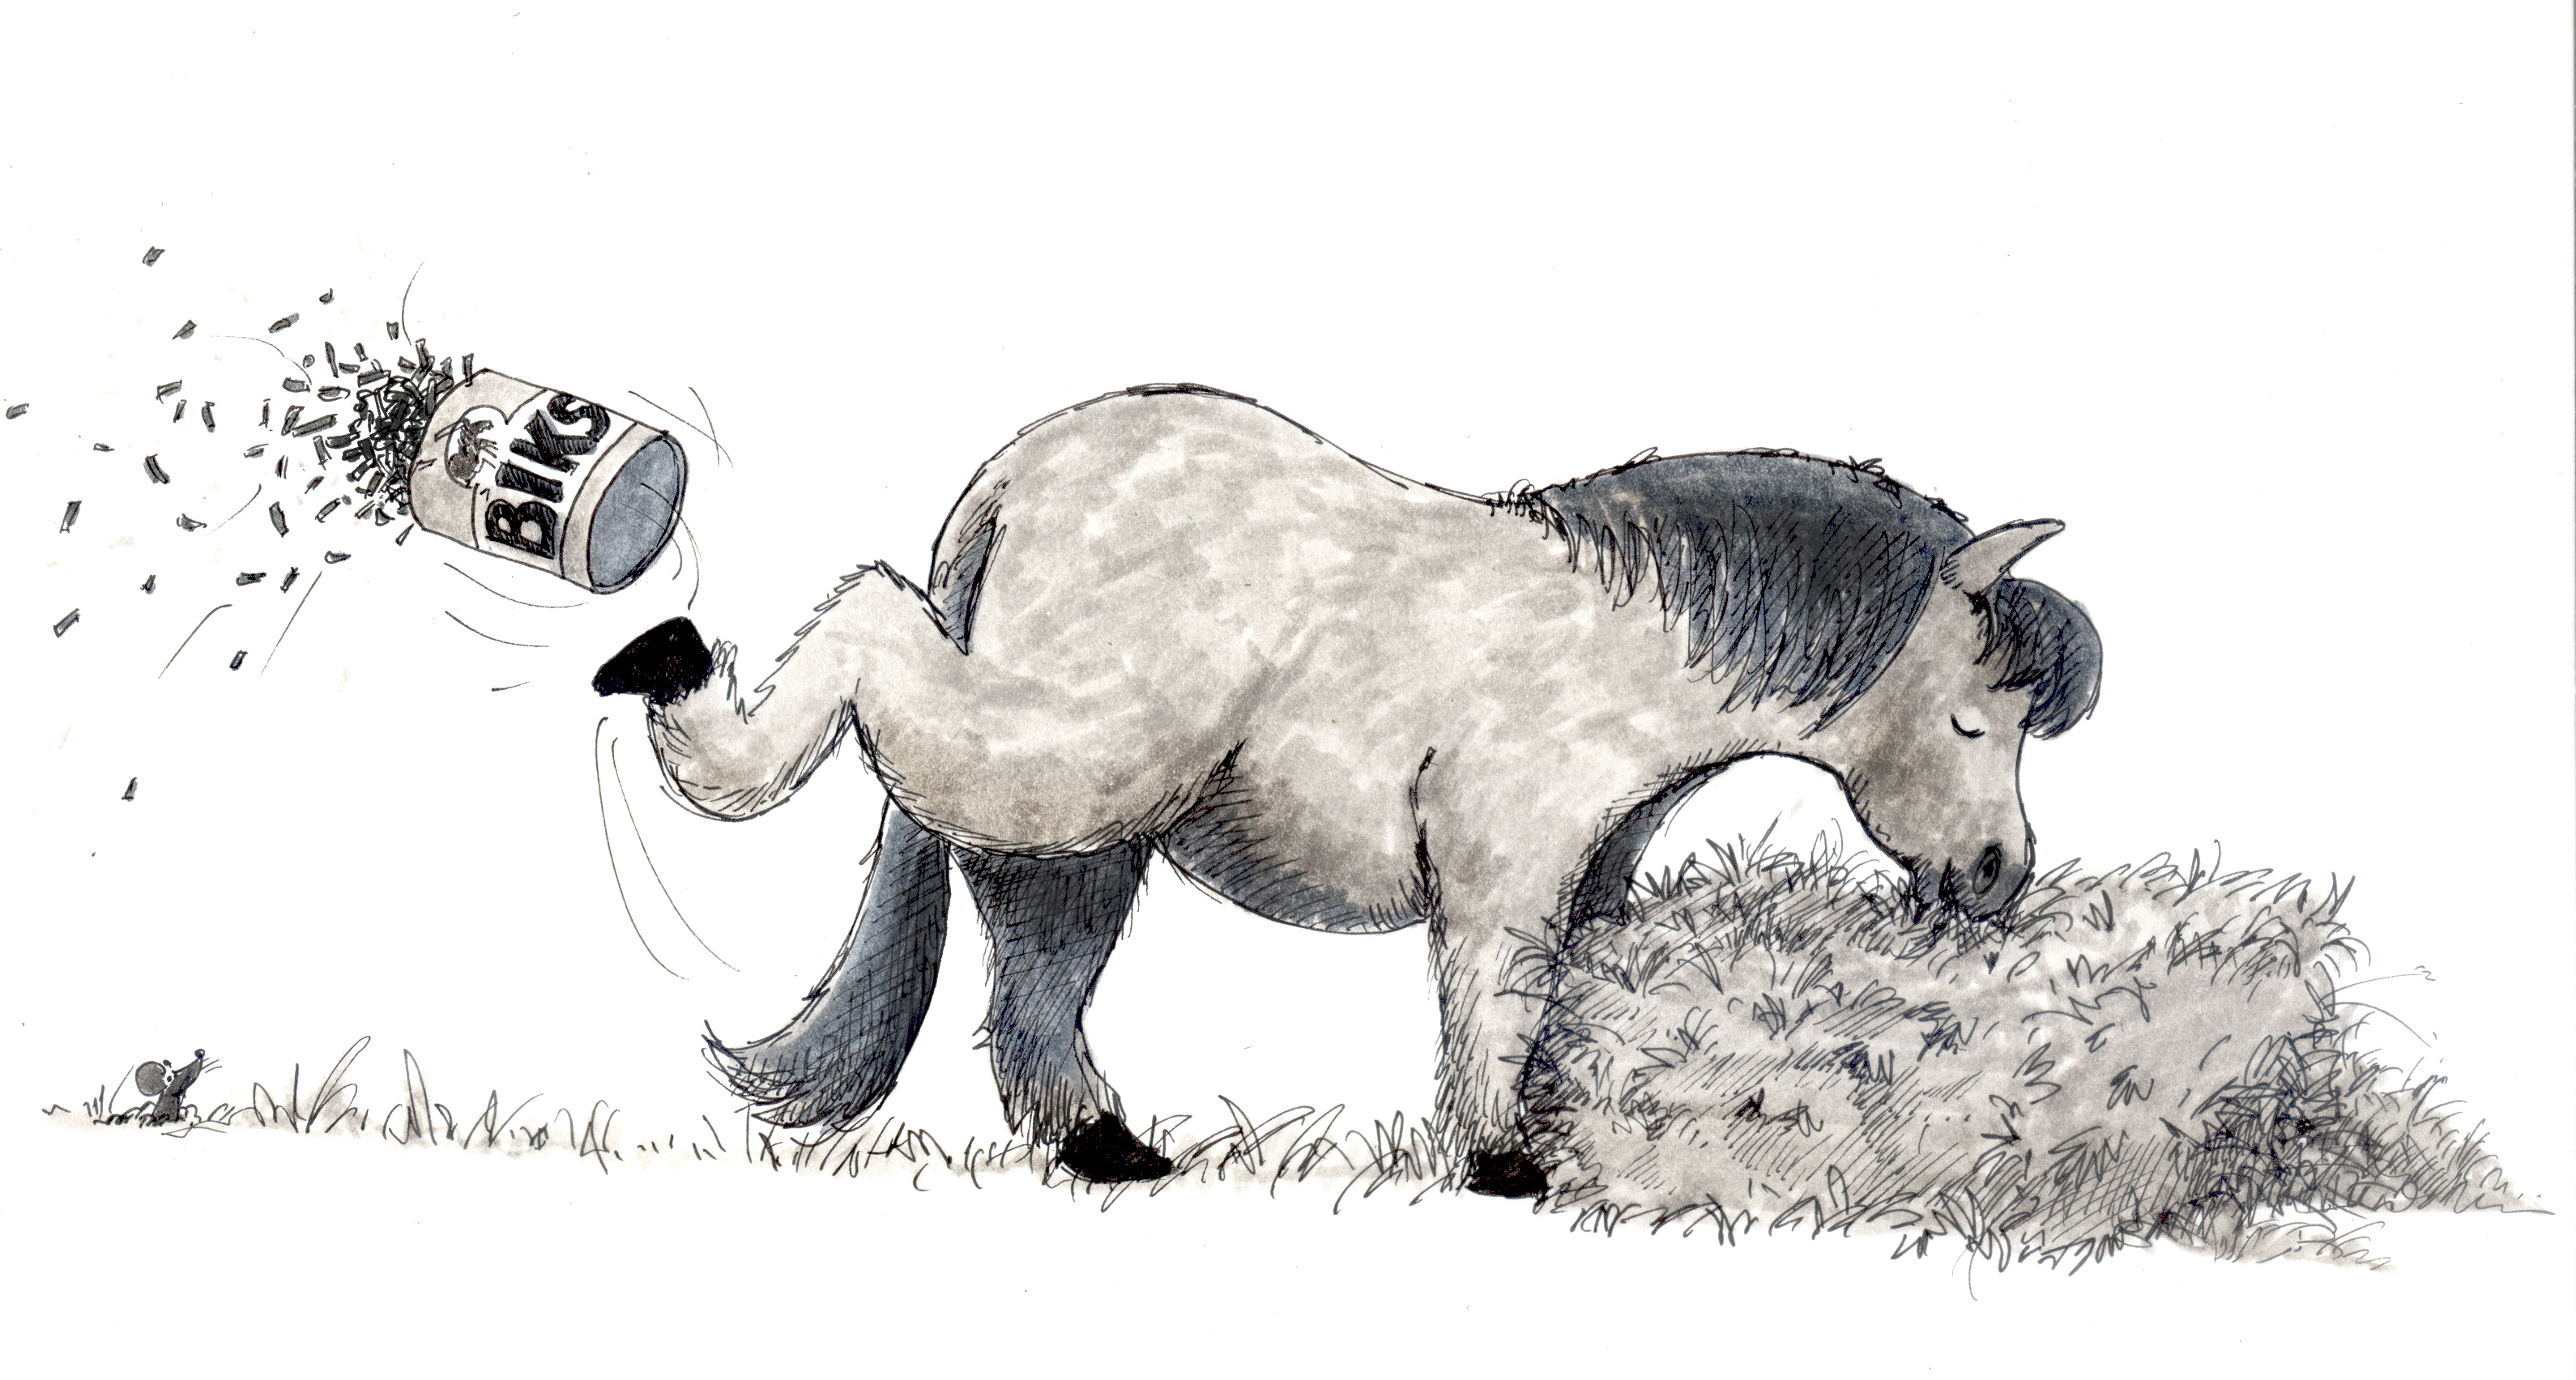
\includegraphics[width=1\linewidth]{img/UW 21 pony.jpg}
    \end{center}   
\begin{multicols}{2}
    
\subsection{Lineaire programmering met een app}
    
    Er zijn verschillende mogelijkheden om het teken- of het rekenwerk aan een computer of een rekenmachine over te laten. Uiteraard is één van deze mogelijkheden voor de leerlingen genoeg. 
    
    \tussentitel{Een online-GeoGebra-app}
    
    Er is een handige GeoGebra-app (Slik, 2011), waar je de randvoorwaarden en de doelfunctie kunt ingeven. Voor de randvoorwaarden moet je de vergelijking van de randen ingeven en met een schuifbalkje kun je dan kiezen welke de `goede kant' is. Voor de doelfunctie geef je een concrete vergelijking: je geeft  een concrete waarde aan de winst of de kosten, zodanig dat de isolijn binnen het scherm valt. Daarna kun je de isolijn verslepen om met de schuifmethode de oplossing grafisch te bepalen. In figuur 1 zie je het schermbeeld voor de laatste opgave, die over het voederen van pony's. Als er veel randvoorwaarden zijn, dan is het toegelaten gebied de doorsnede van veel gekleurde halfvlakken en wordt het soms minder overzichtelijk. Ik probeerde de app ook uit voor de eerste opgave over fietsen en e-bikes; het ging wel maar er waren veel kleuren bij elkaar. In ieder geval laat je best de voorwaarden $x\ge 0, y\ge 0$ weg; die kun je er zelf gemakkelijk bij denken.
    
    \begin{center}
    	\includegraphics[width=\linewidth]{img/linprog fig1.png}
    	\captionof{figure} {Pony's voederen met de GeoGebra-app}
    \end{center}
    
    \tussentitel{Lineair programmeren met Excel}
    
    Een tweede app vind je terug in Excel als invoegtoepassing. De `oplosser' is gebaseerd op de simplexmethode (zie paragraaf 3.3). 
    
    Eerst moet je de `oplosser' activeren in Excel (tenzij dit al gebeurd zou zijn). Hiervoor kies je Bestand en dan Opties. Er opent zich een venster. Hierin kies je Invoegtoepassingen. Je krijgt een lijst met de actieve en de inactieve invoegtoepassingen. Als de Oplosser-invoegtoepassing nog niet actief is, kies je onderaan bij Beheren voor Excel-invoegtoepassingen en klik je op Start. Je krijgt een nieuw venster waarin je Oplosser-invoegtoepassing moet aanvinken. Klik op OK.
    
    Als je nu in het lint op Gegevens klikt, zou de Oplosser er bij moeten staan.
    
    Aan de hand van het voorbeeld van de pony's, laten we zien hoe het werkt.
    
    Eerst moeten we de gegevens invoeren in een Excelblad.
    
    We herhalen even waar het over ging: 
    
    Whiskey heeft per dag $2100\; \mathrm{g}$ koolhydraten  en  $360 
    \; \mathrm{g}$ eiwitten nodig. In één kg biks zit $600\; \mathrm{g}$ koolhydraten en $80 \; \mathrm{g}$ eiwitten. In één kg hooi zit $300\; \mathrm{g}$ koolhydraten en $60\; \mathrm{g}$ eiwitten. Een zak biks van $15 \; \mathrm{kg}$ kost  $\euro 15$; een baal hooi van $20 \; \mathrm{kg}$ kost  $\euro 8$. 
    
    We maken in Excel een tabel met de koolhydraten, de eiwitten en de kostprijs per kg biks en hooi.
    
     \begin{center}
    	\includegraphics[width=1\linewidth]{img/linprog fig2.PNG} 
    	\captionof{figure} {Tabel in Excel}
    \end{center}
    
    In de kolom van de aantallen moeten de variabelen $x$ en $y$ komen. Voorlopig plaats je nullen in deze cellen. Dan selecteer je telkens de cel en met Formules, Naam definiëren geef je de waarden van deze cellen de namen $x$ en $y$. Je ziet voorlopig geen verschil, er staan nog altijd nullen in, maar Excel weet dat dit $x$ en $y$ zijn.
    
    Je voegt een rij met totalen toe. Je gaat onder de kolom van de koolhydraten staan, in de rij van de totalen, en je typt de Excelformule =x*D3+y*D4. Je kunt deze formule dan verslepen voor de andere kolommen (totale hoeveelheid eiwitten; totale prijs per kg). Voorlopig zijn de waarden 0 omdat $x$ en $y$ nog nul zijn.
    
     \begin{center}
    	\includegraphics[width=1\linewidth]{img/linprog fig3.PNG}
    	\captionof{figure} {Tabel in Excel, nu met totalen}
    \end{center}
    
    Aan de cellen met de totalen geef je de namen koolhydraten, eiwitten en kostprijs (zie hoger, met Formules, Naam definiëren).
    
    In de Oplosser vul je de de doelfunctie in (kostprijs). Je kiest voor Min. Je geeft de randvoorwaarden met Toevoegen. Dit is heel kort dankzij de gegeven namen. Je kunt er ook voor kiezen om geen namen te geven aan cellen en alles met de Excelcoördinaten van de cellen doen (bv. D5 voor de cel op de vijfde rij en de D-de kolom van je Excelblad). 
    
    \begin{center}
    	\includegraphics[width=\linewidth]{img/linprog fig4.PNG}
    	\captionof{figure} {De oplosser}
    \end{center}
    
    Je selecteert Simplex LP voor lineaire programmering. De andere twee zijn bedoeld voor gebieden met niet-rechte randen. Ten slotte druk je op Oplossen.
    
    De waarden in de tabel worden hiermee automatisch gewijzigd, zodat je de oplossing kunt aflezen: 0 kg biks, 7 kg hooi. Dan krijgt Whiskey 2100 g koolhydraten en 420 g eiwitten binnen, en het kost Naomi 2,8 euro per dag.
    
    \begin{center}
    	\includegraphics[width=1\linewidth]{img/linprog fig5.PNG}
    	\captionof{figure} {Tabel met de oplossing}
    \end{center}
    
    \tussentitel{Lineair programmeren met een grafische rekenmachine}
    
    Nu de resolutie van het scherm sterk is toegenomen, kan ook de grafische rekenmachine hiervoor gebruikt worden. We verwijzen hiervoor naar Goemaere (2006).
    
    \subsection{Enkele complicaties}
    
    In deze paragraaf willen we enkele speciale zaken bespreken. Is er altijd juist één oplossing? En heeft de oplossing die uit de bus komt, altijd gehele coördinaten? In de economie gaat het vaak over natuurlijke aantallen. Het aantal busjes, het aantal tennisrackets, het aantal fietsen... moeten wel geheel zijn. Toegegeven, je kunt een paard voederen met een niet-geheel aantal kg hooi...
    
    In het volgende voorbeeld komen ook negatieve coëfficiënten voor. Het is niet de bedoeling om dit te interpreteren; bekijk het als een abstract probleem. Maar verderop (2.5) zullen we binnen een context negatieve coëfficiënten zien ontstaan.
    
\end{multicols}
    
\beginwerktekst{Meer dan één oplossing}
    
    \begin{werktekstoef}
    
    \item Teken het toegelaten gebied bepaald door
    
    $$
    \left\{
    \begin{array}{rcl}
         x &\ge &0\\
         y &\ge &0\\
    	 -3x+2y &\le  &7 \\
    	 \, 4x+7y &\le  &39 \\
    	 \, x-3y&\le &5
    	 \end{array}
    \right.
    $$
    \newpage
    
    \emph{Hier is het:}
    
    \begin{center}
   	\includegraphics[width=0.63\linewidth]{img/linprog8.png}
   	\end{center}
    	
    \item Bedenk een winstfunctie zodat $C$ de oplossing is.
    
    \emph{Als de leerling het zich gemakkelijk wil maken, neemt die $y=\mathrm{winst}$, of $ky=\mathrm{winst}$, met $k$ een positieve constante. De isolijnen zijn dan horizontaal. Maar er zijn veel andere isolijnen mogelijk, met een richtingscoëfficiënt tussen die van $BC$ en die van $CD$ in.}
    
    \item Bedenk een winstfunctie zodat er meer dan één oplossing is. Wat doe je $-$ bv. als bedrijfsleider $-$ in zo'n geval?
    
    \emph{Dit is bv. het geval als de isolijnen evenwijdig zijn met $BC$ of met $CD$ of met $AB$. Bijvoorbeeld: $4x+7y=\mathrm{winst}$ (evenwijdig met $BC$). Alle punten van $[BC]$ zijn dan oplossingen. Let op: voor isolijnen evenwijdig met $CD$ is $3x-2y=\mathrm{winst}$  niet goed. Dan zit je ``aan de verkeerde kant'' van de rechte $-3x+2y=7$ en zal er één oplossing zijn, namelijk $(8,1)$. Je moet dus $-3x+2y=\mathrm{winst}$ nemen. Dan zijn alle punten van $[CD]$ oplossingen.}
    
    \emph{Als er meer dan één oplossing is, dan moet de bedrijfsleider kiezen op basis van andere criteria dan winst of kosten.}
    
    \emph{Hou je er rekening mee dat de oplossingen (koppels van) gehele getallen moeten zijn, dan heb je met de isolijnen evenwijdig met $CD$ toch maar één oplossing, namelijk $C$. Het lijnstuk $[CD]$ bevat verder geen punten met gehele coördinaten. Ook het lijnstuk $[BC]$ bevat behalve de eindpunten geen punten met gehele coördinaten. Immers: van $C$ naar $B$ ga je $7$ vakjes naar rechts en $4$ vakjes naar beneden, en $\mathrm{ggd}(7, 4)=1$. Dus: met isolijnen evenwijdig met $BC$ kunnen we er wel voor zorgen dat er twee oplossingen zijn met gehele getallen.}
    
    \item Kun je ook een winstfunctie verzinnen waarbij er geen oplossingen zijn?
    
    \emph{Ik denk het niet. Wat denk jij?}
    
    \end{werktekstoef}
    
\eindewerktekst
    
\begin{multicols}{2}
    
    Wat ook kan gebeuren, is dat het hoekpunt van het toegelaten gebied dat als oplossing uit de bus komt, niet-gehele coördinaten heeft. Als men op zoek is naar de gehele getallen $x$ en $y$ waarvoor de winst maximaal is of de kosten minimaal, dan levert dit hoekpunt niet de oplossing en moet men op zoek gaan naar roosterpunten in de buurt van dat hoekpunt.
    
    Een punt ligt altijd ofwel in een roostervakje, ofwel op een roosterlijn. Je kunt je afvragen of de optimale oplossing met gehele coördinaten altijd één van de vier hoekpunten van het vakje is of één van de twee eindpunten van het roosterlijnstukje is waar het hoekpunt deel van uitmaakt.
    
    Leerlingen kunnen dit onderzoeken door op ruitjespapier (liefst met grote ruiten) een punt te kiezen dat het optimale hoekpunt voorstelt met niet-gehele coördinaten, en dan met een satéstokje verschillende richtingen uittesten voor de isolijnen.
    
    Zij zullen ontdekken dat de hypothese van de hoekpunten van het vakje of de eindpunten van het lijnstukje niet opgaat. Hieronder vind je een tegenvoorbeeld. Het punt $A$ is het hoekpunt dat als oplossing uit de bus komt met de schuifmethode maar de coördinaten zijn niet geheel; het is geen roosterpunt. De hoekpunten van het roostervakje zijn $K,\,L,\,M,\,N$, waarvan $K$ en $L$ binnen het gekleurde toegelaten gebied liggen. Maar je ziet dat punt $B$, ook in het toegelaten gebied, een grotere winst oplevert (de isolijn door $B$ is verder naar rechtsboven dan die door $K$ of $L$).
    
    
    \begin{center}
    	\includegraphics[width=0.7\linewidth]{img/linprog fig6.PNG}
   		\captionof{figure} {Op zoek naar het optimale roosterpunt}
   	\end{center}
    
    Gelukkig gaat het bij realistische problemen meestal over grote getallen, waarbij een oplossing `bij benadering' ook al goed is. Het komt dan niet op één of twee eenheden aan... Er bestaan systematische algoritmen om altijd de beste gehele oplossing te vinden, maar die zijn niet eenvoudig. Je kunt even googelen op `integer linear programming' en dan begrijp je dat we dit hier niet opnemen.
    
\subsection{Lineair programmeren met een parameter}

    In deze paragraaf onderzoeken we wat er gebeurt wanneer we een van de gegeven constanten laten veranderen. Dat doen we door die constante te vervangen door een parameter. We merken dat dit ervoor kan zorgen dat het optimum in een ander hoekpunt van het toegelaten gebied bereikt wordt. En we onderzoeken hoe de optimale waarde afhangt van de waarde van de parameter. 

\end{multicols}

\beginwerktekst{Terug naar het fietsenprobleem} 

    Met de oorspronkelijke gegevens van het fietsenprobleem wordt de optimale oplossing gegeven door punt C in de tweede figuur van de werktekst: 65 fietsen en 175 e-bikes.

    De fietsenhandelaar verlaagt de prijs voor een fiets zodat hij nu maar 100 euro winst maakt per verkochte fiets. De prijs (en winst) voor een e-bike blijft onveranderd. Het is duidelijk dat de fietsenhandelaar hierdoor minder winst zal maken.

\begin{werktekstoef}

    \item Piet zegt dat de maximale winst van de fietsenhandelaar met $\euro 6500$ zal verminderen: elk van de 65 fietsen zal 100 euro minder winst opleveren. Ben je het eens met Piet?
    
    \emph{Neen. Door de gewijzigde winstfunctie, met minder sterk hellende isowinstlijnen, levert niet langer punt C, maar punt D de optimale oplossing.}
    
    \begin{center}
        \includegraphics[width=0.60\linewidth]{img/linprog3bis.png}
    \end{center} 
    
    \emph{De fietsenhandelaar zal dus zijn bestelling aanpassen: $20$ fietsen en $200$ e-bikes. Zijn winst is nu $20 \cdot 100+200\cdot 300=62\,000$ euro. Hij compenseert een deel van het verlies door zijn bestelling aan te passen: minder fietsen en meer e-bikes. In plaats van $6500$ euro maakt hij dus $3500$ euro minder winst}
    
    \item Door de prijs te verhogen of te verlagen, kan de fietsenhandelaar de winst per fiets dus beïnvloeden. Stel de winst per fiets voor door een parameter $p$. De winst wordt nu dus gegeven door $winst=px+300y$. De optimale oplossing hangt af van de waarde van $p$. Welke mogelijkheden zijn er voor de optimale oplossing? Voor welke waarden van $p$ treden ze op?
    
    \emph{Welk punt de optimale oplossing levert, hangt af van de helling van de isowinstlijnen ($-p/300$) en van de helling van de lijnstukken die het toegelaten gebied begrenzen ($ED$: helling $0$; $DC$: $-5/9$; $CB$: $-1$, $BA$: verticaal). Als we aannemen dat de fietshandelaar enkel met strikt positieve waarden van $p$ werkt, dan is de helling van de isowinstlijnen negatief. Als de helling (strikt) tussen $-5/9$ en $-1$ ligt, dan wordt de optimale oplossing gegeven door punt $C$. Dat is als $166,66...<p<300$. Als $p<166,66…$, dan levert punt $D$ de optimale oplossing en als $p>300$, dan bepaalt punt $B$ de optimale oplossing ($100$ fietsen en $140$ e-bikes). Bij beide grenswaarden voor $p$ is er een lijnstuk aan optimale punten.}

    \item Geef de winst van de fietsenhandelaar in functie van p. Maak ook de grafiek van deze functie.
    
    \emph{De winst is}
    \begin{opsomming}
        \item $20 \cdot p + 200 \cdot 300 =60000+20p$ \emph{als} $p \le 166,66...$
        \item $65 \cdot p+175 \cdot 300=52500+65p$ \emph{als} $166,66... \le p \le 300$
        \item $100 \cdot p+140 \cdot 300=42000+100p$ \emph{als} $p \ge 300$
    \end{opsomming}

    \emph{In de grenswaarden maakt het niet uit welk van beide formules je neemt.}
    
    \begin{center}
        \includegraphics[width=0.90\linewidth]{img/linprog3tris.png}
    \end{center} 

\end{werktekstoef}


    

\eindewerktekst

\begin{multicols}{2}

\subsection{Een transportprobleem}
    
    Lineaire programmering kan ook nuttig zijn om problemen op te lossen die er op het eerste gezicht niet als lineaire programmeringsproblemen uitzien. Dat is bv. het geval met bepaalde transportproblemen. In de volgende werktekst bekijken we een transportprobleem dat eigenlijk neerkomt op lineaire programmering met twee variabelen. Het komt uit de Lange \& Kindt (1983).
 \newpage
 
\end{multicols}

\beginwerktekst{Tarwetransport}
    
    \begin{kader}
        Het middenwesten van de Verenigde Staten vormt de graanschuur van de V.S. en van een groot deel van de wereld daarbuiten. Een tarwegroothandelaar heeft pakhuizen in Omaha en Chicago. In het eerste pakhuis heeft hij $50$ vrachtwagenladingen tarwe, in het tweede $40$. 
        
        Hij heeft $20$ wagenladingen verkocht aan Denver, $36$ aan Miami en $34$ aan New York. De transportkosten per wagenlading (in tientallen dollar) zijn gegeven in de volgende tabel.
    \begin{center}
        
    \begin{tabular}{|c|c|c|c|}
        \hline
        &Denver&Miami&New York\\
        \hline
        Omaha&42&55&60\\
        Chicago&36&47&51\\
        \hline
    \end{tabular}
    
    \end{center}
    \end{kader}
    
    \begin{werktekstoef}
    
    \item Teken een gerichte graaf met de vijf steden en pijlen voor de transporten.
    
    \emph{Hier is de graaf. Waar je de knopen tekent, heeft geen belang. Je hoeft geen rekening te houden met de geografische ligging van de steden. Hieronder plaatsten we de knopen zodat de pijlen elkaar niet snijden.}
    
    \begin{center}
        \includegraphics[width=0.50\linewidth]{img/linprog9.png}
    \end{center}
    
    \item Noem $x$ het aantal vrachtwagenladingen van $O$ naar $D$ en $y$ het aantal vrachtwagenladingen van $O$ naar $M$. Duid die aan bij de pijlen van je graaf. Nu liggen alle vrachtwagenladingen vast. Zet bij elke pijl het aantal vrachtwagenladingen, uitgedrukt in $x$ en $y$.
    
    \emph{Zie hieronder.}
    
    \begin{center}
        \includegraphics[width=0.5\linewidth]{img/linprog10.png}
    \end{center}
    
    \item Wat zijn nu de randvoorwaarden waaraan $x$ en $y$ moeten voldoen?
    
    \emph{Alle aantallen vrachtladingen moeten groter dan of gelijk aan nul zijn. Dit geeft:}
    
    $$
    \left\{
    \begin{array}{ccl}
    		 x &\ge  &0 \\
    	  20-x &\ge  &0 \\
    	  y&\ge &0\\
    	  36-y&\ge&0\\
    	  50-x-y&\ge&0\\
    	  x+y-16&\ge&0
    \end{array}
    \right.
    $$
    
    \emph{We kunnen dit vereenvoudigen tot:}
    
    $$
    \left\{
    \begin{array}{cccc}
    		 0&\le x &\le& 20\\
    	  0&\le y&\le&36\\
    	  16&\le x+y &\le &50
    \end{array}
    \right.
    $$
    
    \item{Bepaal de doelfunctie, de kosten in functie van $x$ en $y$.}
    
    $$42x+36(20-x)+55y+47(36-y)+60(50-x-y)+51(x+y-16)=\mathrm{kosten}$$
    $$-3x-y+4596=\mathrm{kosten}$$
    
    \emph{Misschien ben je verbaasd over de mintekens bij $x$ en $y$? Maar $x$ en $y$ zijn maar twee van de zes aantallen vrachtwagenladingen; als die kleiner worden, worden andere aantallen groter...}
    
    \item Teken het toegelaten gebied en los op.
    
    \begin{center}
    	\includegraphics[width=0.70\linewidth]{img/linprog11.png}
    \end{center}
    	
    \emph{Door de negatieve coëfficiënten bij $x$ en $y$ in de kostenfunctie, worden de kosten kleiner als $x$ en $y$ groter worden. Hier moeten we dus de isolijn zoveel mogelijk naar rechtsboven verschuiven. (Het is niet omdat het kosten zijn...) De oplossing is het hoekpunt $(20, 30)$. Dit zijn de aantallen vrachtwagenladingen van Omaha naar Denver en van Omaha naar Miami. Hiermee kunnen alle andere aantallen bepaald worden. De minimale kosten zijn dus: $-3\cdot 20-30+4596=4506$. Omdat de bedragen in tientallen dollar uitgedrukt waren, is dit $\$\; 45 \,060$.}
    
    \end{werktekstoef}
    
\eindewerktekst
    
\begin{multicols}{2}

\subsection{Nog een transportprobleem, nu met een parameter}

We lossen eerst onderstaand probleem zonder parameter op. Daarna zetten we de leerlingen aan het werk met enkele opgaven die parameters vereisen.

\end{multicols}
\newpage
\beginwerktekst{Laptops verschepen}

    \begin{kader}
    Een computerfirma heeft een fabriek in Taiwan en een andere in Vietnam. De Taiwanese fabriek kan hoogstens 600 000 laptops produceren, terwijl de maximale productie in de Vietnamese fabriek op $700\,000$ per jaar ligt. We nemen aan dat er geen verschil in productiekost is. De firma verkoopt de laptops in de Verenigde Staten en in Europa. Volgend jaar verwacht de firma $400\,000$ laptops te verkopen in de Verenigde Staten en $500\,000$ in Europa. Dat zijn dus ook de aantallen die verscheept moeten worden. Voor dat transport zijn er vier transportfirma’s aangetrokken, waarover je in onderstaande tabel de nodige informatie vindt.
    
    \begin{center}
        
    \begin{tabular}{|c|c|c|c|}
        \hline
        Firma&van&naar&kostprijs, per laptop\\
        \hline
        A&Taiwan&Verenigde Staten&8 EUR\\
        B&Taiwan&Europa&10 EUR\\
        C&Vietnam&Verenigde Staten&6 EUR\\
        D&Vietnam&Europa&9 EUR\\
        \hline
    \end{tabular}
    \end{center}
    
    We onderzoeken hoeveel laptops er door elk van de transportfirma’s vervoerd worden als de computerfirma de totale transportkosten minimaliseert.
    
    \end{kader}

    Je hebt ondertussen al voldoende ervaring met problemen van de soort uit de kader. Daarom geven we je niet de opdracht om dit probleem op te lossen. De echte opdracht komt wat verderop, maar vóór we je deze opdracht kunnen geven, moeten we het probleem in de kader oplossen. Een gerichte graaf geeft ons meer zicht op het probleem.
    
    \begin{center}
        \includegraphics[width=0.45\linewidth]{img/linprog graaf.png}
    \end{center} 
    
    We stellen het aantal vervoerde laptops door firma A, B, C en D respectievelijk voor door $a$, $b$, $c$ en $d$ en de totale vervoerskost door $K$. De doelfunctie is dan $K=8a+10b+6c+9d$ en de beperkingen worden gegeven door:
    
    $$
    \left\{
    \begin{array}{rrcl}
         &a+b&\le&600\,000  \\
         &c+d&\le&700\,000 \\
         &a&\ge&0\\
         &b&\ge&0\\
         &c&\ge&0\\
         &d&\ge&0\\
    \end{array}
    \right.
    $$

    We kunnen alles uitdrukken in termen van $a$ en $b$ alleen omdat $a+c=400\,000$ (te verschepen naar de Verenigde Staten) en $b+d=500\,000$ (te verschepen naar Europa). De doelfunctie herleidt zich dan tot $K=2a+b+6\,900\,000$ en de beperkingen worden
    
    $$
    \left\{
    \begin{array}{rrcl}
         &a+b&\le&600\,000  \\
         &a+b&\ge&200\,000 \\
         &a&\ge&0\\
         &b&\ge&0\\
         &a&\le&400\,000\\
         &b&\le&500\,000\\
    \end{array}
    \right.
    $$
    
    We zoeken het optimale punt met de schuifmethode
    
     \begin{center}
        \includegraphics[width=0.68\linewidth]{img/linprogparfig2.png}
    \end{center}
    
    en vinden dat de optimale keuze (met minimale transportkosten) erin bestaat om geen beroep te doen op transportfirma A ($a=0$) en transportfirma B in te zetten om $200\,000$ laptops van Taiwan naar Europa te verschepen. Transportfirma’s C en D verschepen dan respectievelijk $400\,000$ en $300\,000$ laptops.
    
    Nu komt het eerste probleem dat we je willen laten oplossen.
    
    \begin{werktekstoef}    
    
    \item Transportfirma A wil meer laptops verschepen. Misschien lukt dat wel als ze goedkoper worden. Onderzoek of dat het geval is door de prijs voor het vervoer van de laptops van A voor te stellen door een parameter. Geef advies aan de firma over de prijs die ze dan moeten vragen.
    
    \emph{Stel de prijs voor door een parameter $p$. Het toegelaten gebied blijft gelijk, maar de parameter komt wel voor in de doelfunctie: $K=(p-6)a+b+6\,900\,000$. De niveaulijnen hebben vergelijking $b=-(p-6)a+(K-6\,900\,000)$ en zijn dus rechten die schuin of horizontaal lopen, maar nooit verticaal. De constante term in de vergelijking leert ons dat we de niveaulijnen zo ver mogelijk naar onder moeten proberen te schuiven. De waarde van $p$ bepaalt de helling van de niveaulijnen. Deze helling moeten we vergelijken met de helling van de randen van het toegelaten gebied, die horizontaal of verticaal zijn of helling $-1$ hebben. De volgende gevallen treden op (we hebben de twee grensgevallen, met een lijnstuk aan optimale punten, hier weggelaten):}

    \begin{itemize}
        \item \emph{Als de helling van de niveaulijnen kleiner is dan $-1$, dan levert $P_5$ het optimum. Dat is niet gunstig voor firma A: zij zullen niets mogen verschepen. Dit geval treedt op voor $p>7$, zoals in het voorbeeld.}
        \item \emph{Als de helling van de niveaulijnen tussen $-1$ en $0$ ligt, dan levert $P_4$ het optimum. Nu mag firma A $200\,000$ laptops vervoeren. In termen van de parameter betekent dit $6<p<7$.}
        \item \emph{Als de helling van de niveaulijnen groter is dan $0$, dan bepaalt $P_3$ het optimum. Firma A mag dan $400\,000$ computers leveren. Dit komt overeen met $p<6$.}
    \end{itemize}
        
    \emph{We raden de transportfirma daarom aan om zijn prijs tot net onder de $7$ EUR per laptop te laten zakken, en indien verantwoord, zelfs tot net onder de $6$ EUR.}
    \end{werktekstoef}
    
We keren nu terug naar de oorspronkelijke situatie in het kader waarin transportfirma A een prijs van $8$ EUR aanrekent per laptop. De Taiwanese regering wil de computerfirma stimuleren om meer in Taiwan te produceren. Ze beslist daarom om de twee transportfirma’s die vanuit Taiwan opereren, namelijk A en B, een (gelijke) subsidie per getransporteerde PC toe te kennen. Deze firma's kunnen hun prijzen dan verlagen en op die manier aantrekkelijker worden voor de computerfirma.
    
    
    \begin{werktekstoef}
    \setcounter{enumi}{1}                       % om de vorige nummering door te laten lopen
    \item Onderzoek nu eerst of de productie in Taiwan zou toenemen als de regering een subsidie van $3$ EUR per persoon zou toekennen.
    
    \emph{Firma A kan nu transporteren aan een prijs van $5$ EUR per laptop en firma B aan een prijs van $7$ EUR per laptop. De doelfunctie wordt nu gegeven door $K=-a-2b+6\,900\,000$. De niveaulijnen hebben vergelijking $b=-0,5a+(-0,5K+3\,450\,000)$. Bemerk dat we de niveaulijnen nu zoveel mogelijk naar boven moeten schuiven om een zo laag mogelijke kostprijs te krijgen. Het optimum wordt nu gegeven door $P_1$. In plaats van $200\,000$, worden er nu $600\,000$ laptops in Taiwan geproduceerd, wat de maximumcapaciteit is.}
    
    \item Onderzoek de situatie nu verder en stel een advies op voor de Taiwanese regering over de te voeren subsidiepolitiek.
    
    \emph{Stel de subsidie voor door een parameter $s \ge 0$. Dan wordt de doelfunctie gegeven door}
    $$K=(2-s)a+(1-s)b+6\,900\,000.$$ 
    \emph{De niveaulijnen worden gegeven door}
        $$b=-\frac{2-s}{1-s} \cdot a + \frac{1}{1-s} \cdot (K-6\,900\,000)$$ 
    \emph{(behalve als $s=1$).}
    
    \emph{Er zijn verschillende gevallen te onderscheiden (en we laten de randgevallen weer buiten beschouwing):}
         \begin{itemize}
        \item \emph{Als $s<1$, dan moeten we de niveaulijn zo ver mogelijk naar onder schuiven. We kunnen beredeneren dat de helling van de niveaulijn kleiner is dan $-1$, en dat we dus in $P_5$ terechtkomen. Zo’n subsidie heeft dus geen enkel gunstig effect op de productie in de Taiwanese vestiging.}
        \item \emph{Als $s>1$, dan moeten we de niveaulijn zo ver mogelijk naar boven schuiven.}
        
        \begin{itemize}
            \item \emph{Zolang $s<2$, hebben de niveaulijnen een positieve helling en is $P_6$ optimaal. De productie in Taiwan neemt dan toe van $200\,000$ naar $500\,000$.}
            \item \emph{Als $s>2$, dan ligt de helling van de niveaulijnen tussen $-1$ en $0$. Het optimum wordt nu bereikt in $P_1$. De productie in Taiwan ligt dan op $600\,000$.}
        \end{itemize}
    \end{itemize}
    \emph{We raden de Taiwanese regering aan om een subsidie van net iets meer dan $1$ EUR per getransporteerde laptop te geven. Dat heeft een groot effect op de productie in Taiwan. Er is nog een bijkomend effect als de subsidie stijgt tot iets meer dan $2$ EUR, maar dat bijkomende effect is bescheidener.}    
    \end{werktekstoef}
    
\eindewerktekst

\begin{multicols}{2}

\subsection{Interpretatie in 3D van lineaire programmering met twee veranderlijken}
    
    De doelfunctie is een functie van twee veranderlijken. De grafiek van een functie van twee veranderlijken is een oppervlak in de ruimte. Het vlak met de $x$- en de $y$-as leggen we plat op de tafel. Het beeld van het koppel $(x,y)$ bekijken we als de (positieve of negatieve) hoogte van een punt boven of onder de tafel. Al deze punten vormen de grafiek van de functie: een oppervlak in de ruimte. In het geval van de doelfunctie bij lineaire programmering is de functie van de eerste graad. De grafiek is dan een vlak. Net zoals de grafiek van een eerstegraadsfunctie van één veranderlijke een rechte is, is de grafiek van een eerstegraadsfunctie van twee veranderlijken een vlak. 
    
    Laten we dit even illustreren aan de hand van het tweede voorbeeld dat we bekeken hebben: 
         $$
    \left\{
    \begin{array}{rrcl}
    	
          &\;\;\;\;0\;\;\;\;\le \;\;\;\;x &\le &10 \\
          &\;\;\;\;0\;\;\;\;\le \;\;\;\;y &\le & 8 \\
    	  &x+2y &\le  &18 \\
    	  &x+y &\le  &13 \\
    	  &200x+300y&=&\mathrm{winst}
    	
    \end{array}
    \right.
    $$ 

    De doelfunctie is $\mathrm{winst}=200x+300y$. Als we nu even de winst uitdrukken in honderdtallen euro's en met $z$ noteren, krijgen we $z=2x+3y$. Hier is de grafiek, getekend met GeoGebra (3D).
    
    \begin{center}
    	\includegraphics[width=\linewidth]{img/linprog fig7.png}
    	\captionof{figure} {Grafiek van de doelfunctie}
    \end{center}
    	
    In het $xy$-vlak tekenen we nu het toegelaten gebied.
    
    \begin{center}
    	\includegraphics[width=\linewidth]{img/linprog fig8.PNG}
    	\captionof{figure} {Grafiek van de doelfunctie met het toegelaten gebied}
    \end{center}
    	
    Enkel het stuk van de grafiek boven de punten van het toegelaten gebied, zijn van belang. Het toegelaten gebied bepaalt een prisma, dat bovenaan afgesneden is door de grafiek van de doelfunctie. We zoeken boven welk punt van het toegelaten gebied de hoogte (de winst) maximaal is.
    
    \begin{center}
    	\includegraphics[width=\linewidth]{img/linprog fig9.png}
    	\captionof{figure} {Prisma bepaald door het toegelaten gebied}
    \end{center}
    	
    De isolijnen, rechten van gelijke winst, zijn nu te interpreteren als niveaulijnen, net zoals bij een kaart van een (berg)landschap. Omdat het landschap een schuin vlak is, zijn de niveaulijnen evenwijdige rechten.
    
    \begin{center}
    	\includegraphics[width=\linewidth]{img/linprog fig10.png}
    	\captionof{figure} {De isolijnen als niveaulijnen}
    \end{center}
    
    Een bovenaanzicht van deze figuur is precies de vlakke figuur uit de werktekst `nu helemaal zelf'.

\section{Drie of meer veranderlijken}
	
	Met deze paragraaf willen we toch even buiten de oevers van de nieuwe eindtermen gaan. Dit is geen leerstof meer in economie-moderne talen of bedrijfswetenschappen. Als je dit in deze klassen ter sprake brengt, moet je natuurlijk beseffen dat deze leerlingen geen analytische ruimtemeetkunde hebben bestudeerd. Het zou ook een uitbreiding kunnen zijn voor (sommige) leerlingen in wiskundeklassen (bv. in economie-wiskunde, als voorbereiding op hogere economiestudies). De simplexmethode (paragraaf 3.3) kan dan gezien worden als een toepassing op het oplossen van stelsels met de methode van Gauss-Jordan.
	
	Lineaire programmeringsproblemen met twee veranderlijken kunnen grafisch worden opgelost (zie vorige paragraaf): het toegelaten gebied is een deel van het vlak begrensd door rechte lijnstukken en de lijnen van gelijke opbrengst of kost zijn evenwijdige rechten. De grafische methode werkt hier prima. 
	
	Voor drie veranderlijken kan de grafische methode worden veralgemeend. Het toegelaten gebied is nu een stuk van de ruimte, begrensd door vlakke veelhoeken. In plaats van evenwijdige lijnen van gelijke opbrengst of kost heb je nu evenwijdige vlakken. Leerlingen die ook analytische ruimtemeetkunde op hun leerstofplank hebben, weten (of zullen weten) dat een vergelijking van de eerste graad in drie veranderlijken inderdaad een vlak voorstelt in de ruimte. Een ongelijkheid van de eerste graad in drie veranderlijken stelt een `halfruimte' voor, het deel van de ruimte aan één kant van dat vlak. Leerlingen die geen ruimtemeetkunde krijgen, zullen dit hier zien als een veralgemening van de situatie met twee veranderlijken, een dimensie hoger, zonder er diep op in te gaan. Je kunt dan op GeoGebra rekenen om deze vlakken te tekenen... 
	
	Het grafisch oplossen houdt hier wel op. Voor vier of meer veranderlijken hebben wij $-$ normaal gezien toch $-$ niet genoeg hyperruimtelijk voorstellingsvermogen om het probleem op te lossen op een tekening. Hiervoor is er de simplexmethode, die gebruik maakt van matrices en stelsels. Ook dit vormt een mooie verbinding met een ander stuk leerstof. 
	
	Als je de kennismaking met lineaire programmering enkel wilt uitbreiden met een exemplarisch voorbeeld met drie veranderlijken, kun je je beperken tot 3.1 (en eventueel 3.2). Als je een mooie toepassing wilt aanbrengen van matrices en stelsels, en een inkijk wilt geven in een algoritme (computationeel denken...) dat de basis vormt voor het oplossen van lineaire programmeringsproblemen door computers, met heel wat meer variabelen en ongelijkheden, dan kun je gebruik maken van de korte introductie tot de simplexmethode in de paragrafen (3.2 en) 3.3. We leggen meer de nadruk op het begrijpen van de simplexmethode en de link met de tekening, dan op het `inoefenen' van het algoritme.
	
	We beperken ons in deze paragraaf tot problemen waarbij een eerstegraadsfunctie \emph{gemaximaliseerd} moet worden. Dus: tot winst en niet kosten.
	
\subsection{Drie veranderlijken}
	
	In deze werktekst lossen de leerlingen een lineaire programmeringsprobleem op in de ruimte. Ze denken hierbij na over de dimensiesprong van het vlak naar de ruimte. De opgave over geneesmiddelen komt uit de Lange \& Kindt (1983).
	
\end{multicols}

\beginwerktekst{Drie geneesmiddelen}

    \begin{kader}
        Dat het voor een farmaceutisch bedrijf belangrijk is om op korte tijd grote hoeveelheden vaccins of geneesmiddelen te kunnen produceren, is sinds de coronacrisis voor iedereen duidelijk geworden.

        Een farmaceutisch bedrijf moet binnen een tijdsbestek van 190 uur grote hoeveelheden van drie geneesmiddelen X, Y en Z maken. Het duurt 3 uur om $1\,000$ flesjes X te maken; 2 uur om $1\,000$ flesjes Y te maken en 4 uur om $1\,000$ flesjes Z te maken. Het bedrijf kan niet meer dan $30\,000$ flesjes X, $40\,000$ flesjes Y en $20\,000$ flesjes Z maken. Per $1\,000$ flesjes X maakt het bedrijf € 12 winst; per $1\,000$ flesjes Y is de winst € 17 en per $1\,000$ flesjes Z is de winst € 9.
    \end{kader}

    \begin{werktekstoef}
    
	\item Noteer het vraagstuk als een stelsel van drie ongelijkheden en een winstfunctie. Noteer het aantal duizendtallen flesjes X, Y en Z als $x, y$ en $z$.
	
	\emph{Dit geeft:}
	
	$$
	\left\{
	\begin{array}{ccl}
		
		3x+2y+4z  &\leq  &190 \\
		\;\;\;\;\;\;\;\;0\;\;\le \;\;\;\;x\;    \;\;   &\leq  &30\\
		\;\;\;\;\;\;0\;\;\le \;\;\;\;y  \;     &\leq & 40\\
		\;\;\;\;\;\;0\;\;\le\;\;\;\;	 z       &\leq & 20\\
		12x+17y+9z &= & \text{winst}
		
	\end{array}
	\right.
	$$
	
	\item De `toegelaten ruimte', tegenhanger van het toegelaten gebied bij twee veranderlijken, bestaat uit alle punten $(x,y,z)$ van de ruimte $\mathbb{R}^3$ die voldoen aan alle ongelijkheden van het probleem. Hieronder zie je de toegelaten ruimte bij dit probleem. Leg de betekenis uit van elk zijvlak.
	
	\begin{center}
		\includegraphics[width=0.4\linewidth]{img/linprog12.png}
	\end{center}
	
	\emph{De balk wordt gevormd door de ongelijkheden $0\leq x \leq 30$ (de punten moeten tussen voor- en achtervlak liggen), $0\leq y \leq 40$ (de punten moeten tussen linker- en rechtervlak liggen) en $0\leq z\leq 20$ (de punten moeten tussen onder- en bovenvlak liggen). De ongelijkheid $3x+2y+4z\leq 190$ bepaalt een schuin vlak waarmee een hoek van de balk wordt afgesneden. De punten moeten `onder' dit schuine vlak liggen, in de halfruimte waar ook het punt $(0,0,0)$ ligt.}
	
	\item Bij drie veranderlijken hebben we vlakken van gelijke winst in plaats van gelijke-winstlijnen. Je kunt de vorige figuur in GeoGebra openen (\url{https://www.geogebra.org/m/qypmsusw}) en de gelijke-winstvlakken erbij tekenen. Hiervoor geef je het voorschrift van de winstfunctie in in de invoerregel. In plaats van het woord `winst' of `opbrengst', gebruik je één letter, bv. $w$. GeoGebra zal hier een schuifbalk voor maken. Verander de eigenschappen van de schuifbalk zodat die realistische winstwaarden kan aannemen. Let op: de schuifbalk zie je niet in het 3D-venster. Om die te zien, open je ook een 2D-venster of het algebravenster. 
	
	\emph{Leerlingen geven in: $12x+17y+9z=w$ en GeoGebra maakt een schuifbalk voor $w$. Om een realistisch interval te vinden voor de variabele $w$, kunnen ze bv. de winst berekenen voor het weggesneden hoekpunt $(30, 40, 20)$ van de balk: $€ 1\,220$. Een interval $[0, 1\,200]$ of $[0, 1\,500]$ zal zeker ruim genoeg zijn.}
	
	\begin{center}
		\includegraphics[width=0.65\linewidth]{img/linprog13.png}
		
	\end{center}
	
	
	\begin{center}
		\includegraphics[width=0.65\linewidth]{img/linprog14.png}
	\end{center}
	
	\item Bepaal door te schuiven met het gelijke-winstvlak in welk punt van de toegelaten ruimte de winst maximaal is. Voor de duidelijkheid kun je eventueel de snijlijnen van het gelijke-winstvlak met de zijvlakken van de toegelaten ruimte zichtbaar maken (met de knop `doorsnede van oppervlakken').
	
\begin{multicols}{2}

		\begin{center}
			\includegraphics[width=\linewidth]{img/linprog15.png}
			
			\includegraphics[width=\linewidth]{img/linprog16.png}
		\end{center}

	\end{multicols}
	
	\emph{Het hoekpunt met maximale winst (schuifbalk zo ver mogelijk naar rechts zonder de toegelaten ruimte volledig te verlaten) is op de verticale ribbe}
	
	$$
	\left\{
	\begin{array}{l}
		
		x=30\\
		y=40
		
	\end{array}
	\right.
	$$
	
	\emph{en in het schuine vlak $3x+2y+4z=190$. De $z$-coördinaat vinden we door $3\cdot 30+2\cdot 40+4z=190$ op te lossen naar $z$. Het is dus het punt $(30, 40, 5)$.}
	
	\item Formuleer de oplossing van het probleem.
	
	\emph{Als het farmaceutisch bedrijf zoveel mogelijk winst wil maken, moet het $30\, 000$ flesjes $X$, $40\,000$ flesjes $Y$ en $5\,000$ flesjes $Z$ produceren. De winst is dan: $12\cdot 30 + 17\cdot 40+ 9\cdot 5=1\,085$ euro.}
	
	\emph{Hier vind je een GeoGebrafiguur met de schuifbalk en het veranderlijke vlak van gelijke winst erbij: \url{https://www.geogebra.org/m/gnzg9k6z}}
	
    \end{werktekstoef}

\eindewerktekst

\begin{multicols}{2}
	
\subsection{Wandelen langs de ribben}
	
	Het tekenen van gelijke-winstvlakken is lastiger dan de gelijke-winstlijnen in het geval van twee veranderlijken. Met GeoGebra lukt dit nog wel. Bij vier of meer veranderlijken is dit echter onbegonnen werk. We zijn op zoek naar een andere methode.
	
	Als er maar één oplossing is, dan is deze oplossing altijd een hoekpunt van de toegelaten ruimte. Als er meer oplossingen zijn, omdat de gelijke-winstvlakken evenwijdig zijn aan een ribbe of een zijvlak van de toegelaten ruimte, dan is er steeds een hoekpunt bij.
	
	Dit leidt tot de volgende methode: we berekenen de winst in elk hoekpunt van de toegelaten ruimte en we zien waar de winst het grootst is.
	
	Voor problemen met veel veranderlijken en een groot aantal hoekpunten, is dit niet zo efficiënt. Het kan korter. We kunnen vertrekken in één hoekpunt, bv. $(0, 0, 0)$, en telkens `wandelen' langs een ribbe naar een `naburig' hoekpunt waar de winst groter is.
	
	\tussentitel{Bij het farmaceutisch voorbeeld}
	
	Wat zou dit geven in het voorbeeld van de vorige werktekst, met de geneesmiddelen X, Y en Z?
	
	$$
	\left\{
	\begin{array}{ccl}
		
		3x+2y+4z  &\leq  &190 \\
		x\;\;\;\; \;\; \;\;\;\;\;\; \;\;\;\; \;\;   &\leq  &30\\
		\;\;\;\;\;\;\;\;	\;\;y \;\; \;\;\;\;\;\;     &\leq & 40\\
		\;\;\;\;\;\;\;\;\;\;\;\;\;\;\;\;\;\;\;\;	\;\;\;\;z       &\leq & 20\\
		12x+17y+9z &= & \text{winst}
		
	\end{array}
	\right.
	$$

	\begin{opsomming}
		\item We starten in $(0, 0, 0)$ waar de winst $0$ is. 
		\item We kunnen bv. langs de $y$-as wandelen. Op basis van de coëfficiënt $17$ in de winstfunctie valt daar wel iets voor te zeggen: elke stap waardoor $y$ een eenheid groter wordt, levert 17 euro extra winst op, terwijl dit voor de $x$-as maar 12 euro is. We komen in hoekpunt $(0, 40, 0)$ en de winst is hier 680 euro.
		
		\item Nu kunnen we naar hoekpunt $(30, 40, 0)$ wandelen. Daar is de winst 1040 euro.
		
		\item Nu mogen we niet naar $(30, 0, 0)$ wandelen want daar is de winst weer lager (namelijk 360). We wandelen `naar boven', naar $(30, 40, 5)$, en daar is de winst opgeklommen tot $1\,085$ euro.
		
		\item We stoppen want in de naburige hoekpunten $(30, 10, 20)$ en $(10, 40, 20)$ is de winst lager.
	\end{opsomming}

	\begin{center}
		\includegraphics[width=0.9\linewidth]{img/linprog fig11.PNG}
		\captionof{figure} {Wandeling naar een maximale winst}
	\end{center}
	
	Bij een ingewikkelder probleem kan het wandelen van het ene naar het andere hoekpunt een grote besparing betekenen vergeleken met het berekenen van de winst in \emph{elk} hoekpunt. 
	
	\tussentitel{Leidt zo'n wandeling altijd naar een oplossing?}
	
	Is het zeker dat er bij dat wandelen altijd een oplossing (een punt met maximale winst) uit de bus komt? 
	\begin{center}
		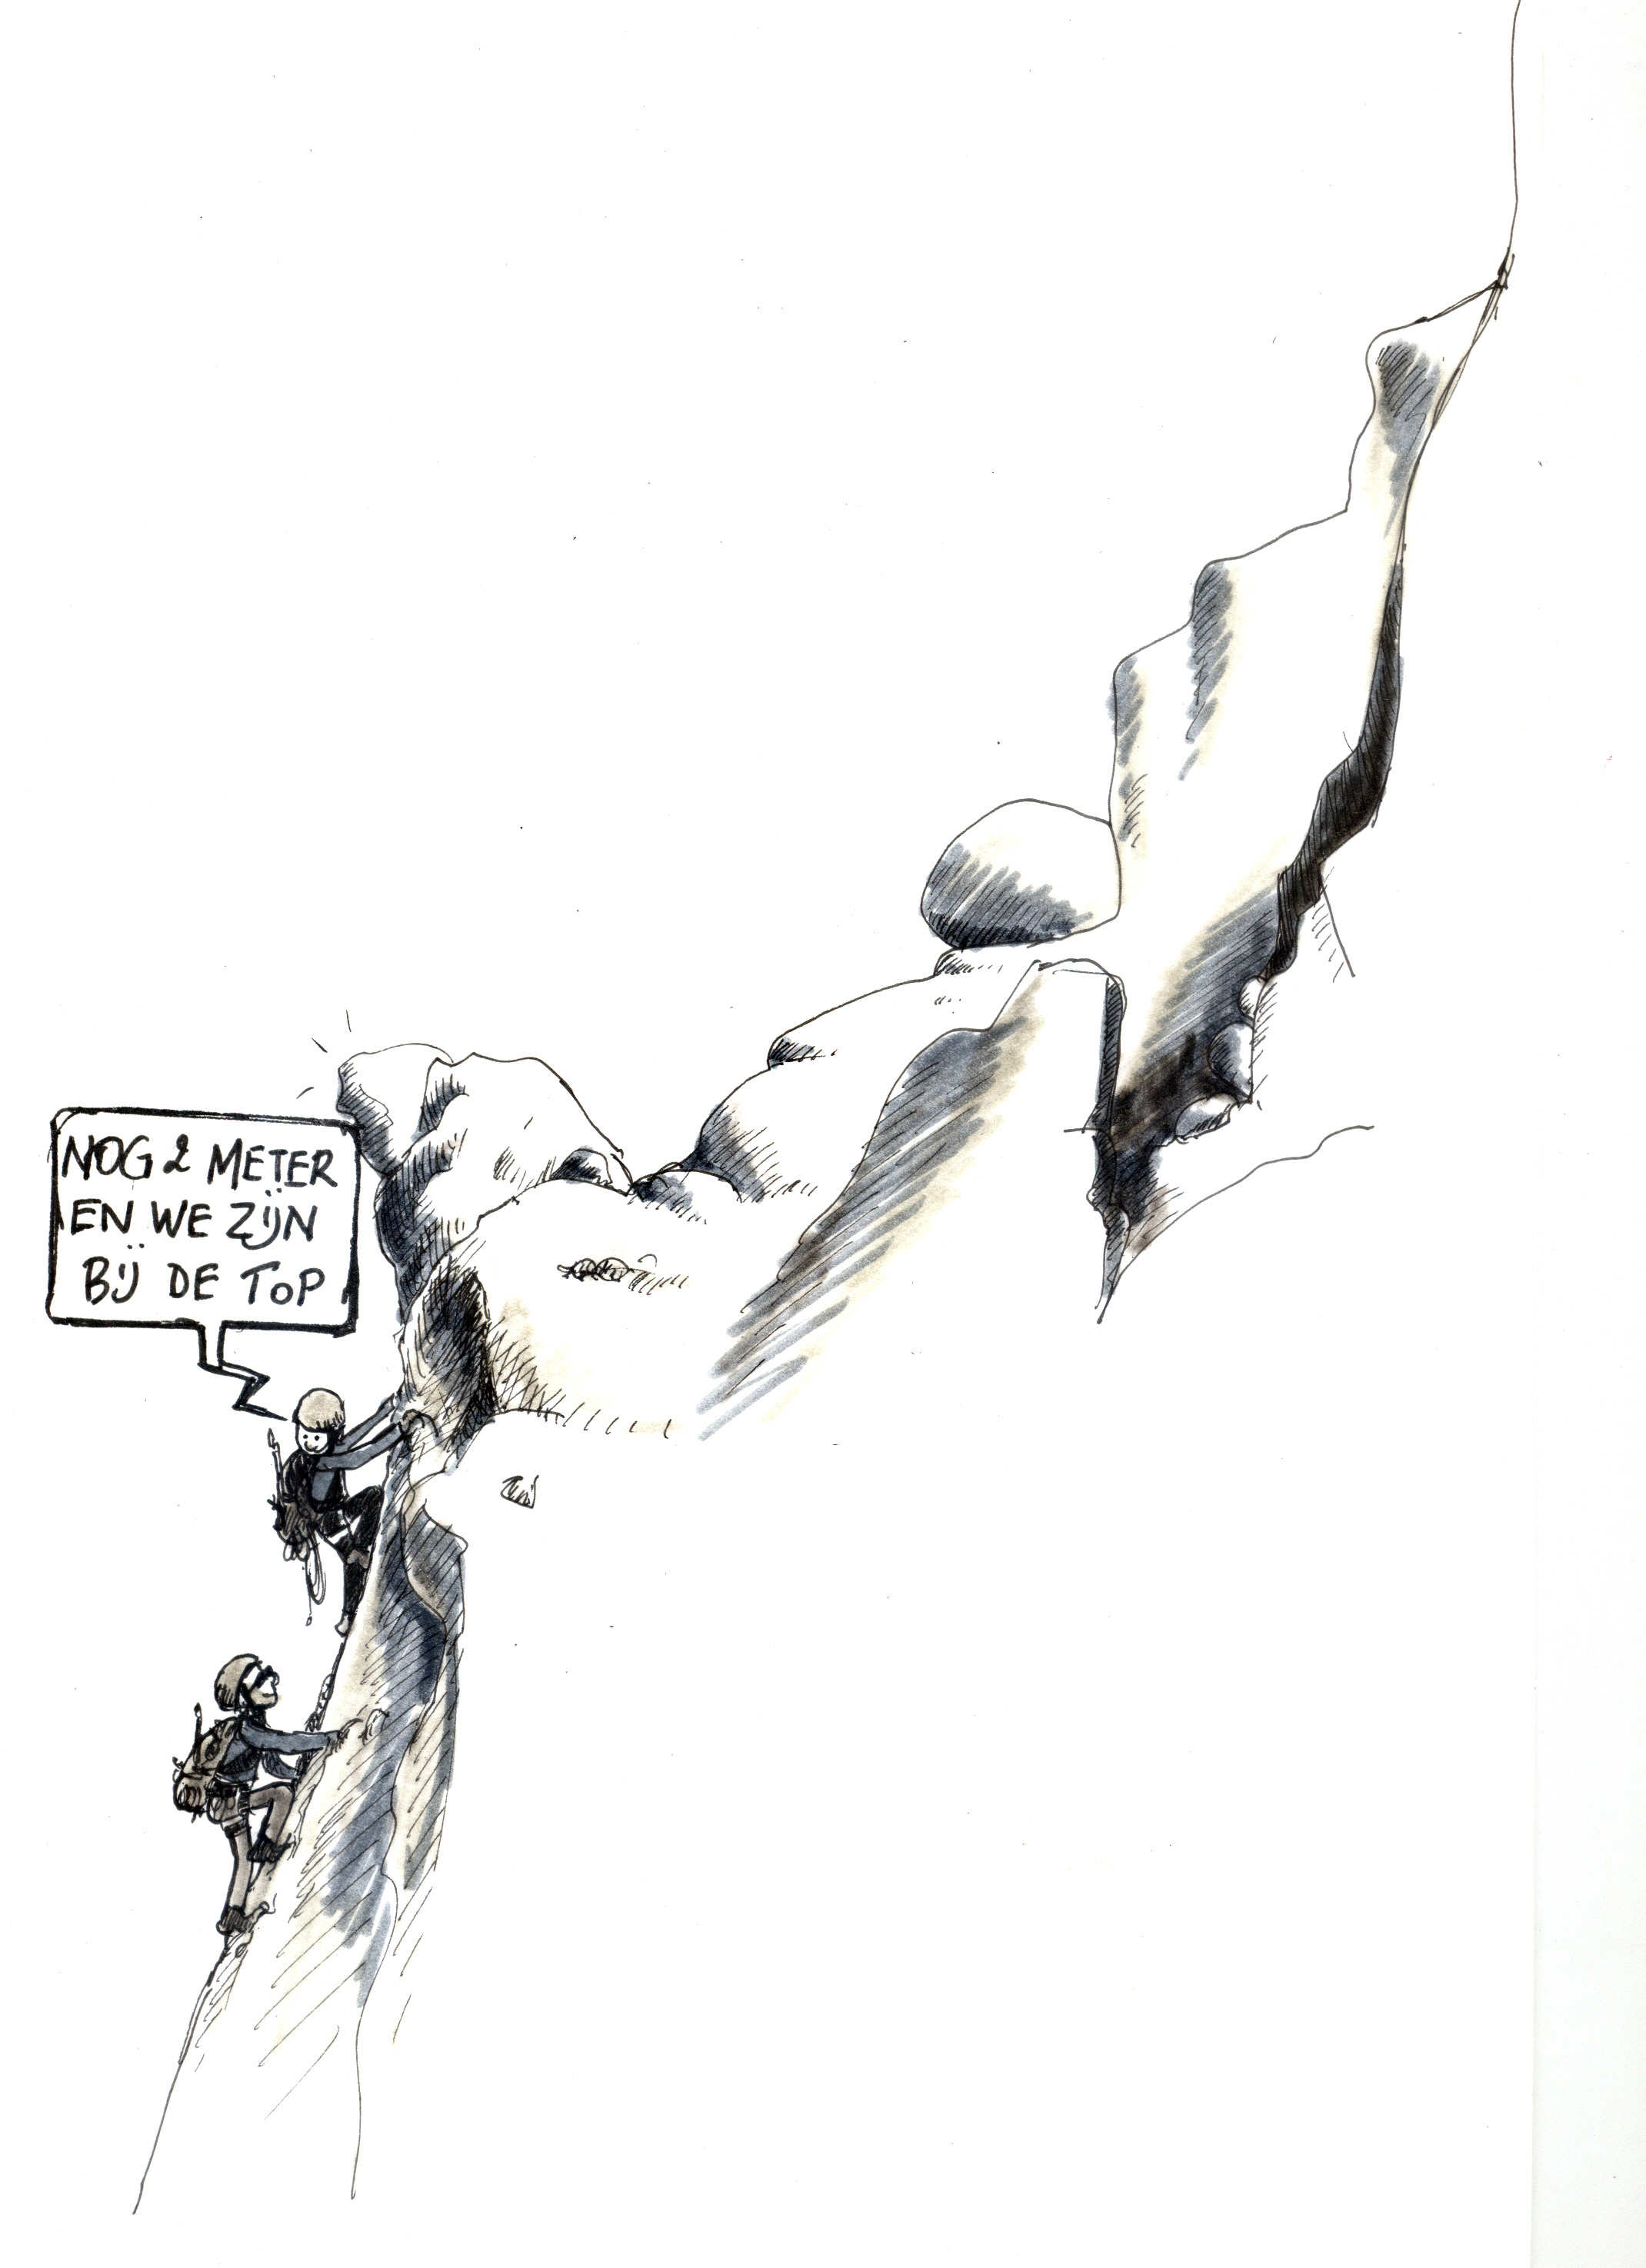
\includegraphics[width=1\linewidth]{img/UW 21 berg.jpg}
		
	\end{center}
	Stel even dat de gelijke-winstvlakken horizontaal zijn (of, wat op hetzelfde neerkomt, draai de hele toegelaten ruimte zo dat die vlakken horizontaal komen te liggen). Wandelen naar een hoekpunt met grotere winst betekent dan: naar een hoger gelegen hoekpunt klimmen. Als de toegelaten ruimte uit `één berg' bestaat, zoals in figuur 12 links, dan leidt het klimmen zeker tot een `oplossing'. Als de toegelaten ruimte verscheidene `toppen' heeft, leidt het klimmen niet noodzakelijk tot een `oplossing'. Het verschil tussen beide figuren is dat de toegelaten ruimte links `convex' is en rechts niet.
	
	\begin{center}
		\includegraphics[width=0.9\linewidth]{img/linprog fig12.png}
		\captionof{figure} {Eén of meer `toppen'}
	\end{center}

	Een figuur (in het vlak, in de ruimte of in een hogerdimensionale ruimte) is \emph{convex} wanneer voor elk paar punten $P$ en $Q$ binnen de figuur, het lijnstuk $[PQ]$ helemaal binnen de figuur ligt.
	
	De oplossingenverzameling van een eerstegraadsongelijkheid is altijd convex. Bv. in de ruimte is dat een `halfruimte', het deel van de ruimte aan één kant van een vlak. Als $P$ en $Q$ aan één kant van een vlak liggen, dan ook het verbindingslijnstuk.
	
	
	De doorsnede van convexe verzamelingen is altijd convex. Dit kun je gemakkelijk aantonen. 
	
	Welnu, de toegelaten ruimte is de oplossingenverzameling van een stelsel van eerstegraadsongelijkheden, dus de doorsnede van convexe verzamelingen, en dus convex.
	
	We mogen dus op onze twee oren slapen: met de methode van het wandelen langs de ribben, vind je altijd een oplossing. Deze oplossing hoeft niet uniek te zijn, net zoals in het vlak (zie paragraaf 2.4). De volgende oefening, geïnspireerd door de Lange en Kindt (1983), is een voorbeeld van een lineair programmeringsprobleem met drie variabelen en meer dan één oplossing.
	
\end{multicols}
	
	
	
\beginwerktekst{Oefening}

    Hieronder zie je een lineair programmeringsprobleem. De toegelaten ruimte is erbij afgebeeld en de coördinaten van de hoekpunten staan erbij:

    $$
    \left\{
    \begin{array}{ccl}
	
	    \;\;\;\;\;\;\;\frac{x}{2}\;\;+y\;\;+z  &\leq  &13 \\
	    \;\;\;\;\;\;\;\;\;\;\;\;\;\;\;\;\;y\;\;+2z &\leq &18 \\
	    0 \;\; \le \;\; x\;\;\;\;\;\;\;\;\; \;\;\;\;    &\leq  &15\\
	    0\;\;\le \;\;\; \;\;y\;\;\;\;\;\;\;	 \;\;     &\leq & 10\\
	    0\;\;\le\;\;\;\;\;\;\;\;\;\;\;	z\;\;\;       &\leq & 8\\
	    50x+200y+300z &= & \text{winst}
	
    \end{array}
    \right.
    $$

	\begin{center}
		\includegraphics[width=0.75\linewidth]{img/linprog17.png}
	\end{center}

    Wandel van hoekpunt naar hoekpunt via ribben en los het lineaire programmeringsprobleem op.

    \emph{Het vertrekpunt van de wandeling hoeft niet $(0, 0, 0)$ te zijn; de leerlingen kunnen starten waar ze willen en zodra er geen buurhoekpunten zijn met hogere winsten zijn ze klaar.}

    \emph{Als we toch in $(0,0,0)$ starten, gaan we naar H (vanwege de hoge coëfficiënt bij $z$ in de winstfunctie). In $H$ is de winst $2\,400$. Vanuit $H$ kunnen we naar $G$ (winst $2\,800$) of naar $L$ (winst $2\,900$) wandelen. We gaan dus naar $L$. De `beste' buur van $L$ is $K$, met winst $3\,100$. De enige buur van $K$ waar we nog niet gepasseerd zijn, is $F$. Daar is de winst ook $3\,100$. Dit betekent dus dat de vlakken van gelijke winst evenwijdig zijn met de ribbe $[KF]$. Er zijn dus oneindig veel oplossingen: alle punten van deze ribbe.}

    \emph{Misschien vraag je je af: kunnen de vlakken van gelijke winst ook evenwijdig zijn met een heel zijvlak? Dat zou dan $KFG$ of $KFECBML$ moeten zijn, want in de punten van $[KF]$ is de winst alvast maximaal. Maar dat is hier niet het geval, want we weten al dat de winst in $L$ en in $G$ kleiner is dan $3\,100$.}

\eindewerktekst

\begin{multicols}{2}

\subsection{De simplexmethode}
	
	We hernemen het aanvangsprobleem over fietsen en e-bikes. We kennen de oplossing al, maar juist daarom is dat probleem geschikt om hiermee op zoek te gaan naar een louter algebraïsche oplossingswijze.
	
	Het probleem is
	
	$$
    \left\{
    \begin{array}{ccl}
    	
    	0\;\; \le \;\;\;\;\; x &\le &100 \\
    	0\;\;\le \;\;\;\;\; y &\le &200 \\
    	\;\;\;5x+9y &\le  &1900 \\
    	\;\;\;x+y &\le  &240\\
    	200x+300y &= &\mathrm{winst}
    	
    \end{array}
    \right.
    $$  

	\tussentitel{Spelingsveranderijken}
	
	Bij de simplexmethode moeten de variabelen altijd groter dan of gelijk zijn aan nul. De voorwaarden $0\le x, \;0\le y$ zullen we er niet meer bij schrijven maar stilzwijgend veronderstellen.
	
	Voor een stelsel van eerstegraads\emph{on}gelijkheden kennen we geen algebraïsche oplossingsmethode, maar wel voor een stelsel van eerstegraads\emph{ver}gelijkingen. Daarom maken we van elke ongelijkheid een vergelijking. We doen dat door \emph{spelingsveranderlijken} toe te voegen (in het Engels: `slack variables'). De spelingsveranderlijken geven aan wat het verschil is tussen het rechterlid en het linkerlid van de ongelijkheid. We noemen ze $s_1, s_2, s_3, s_4$.
	
	$$
	\left\{
	\begin{array}{rccl}
		
		 x & +\ \ \ s_1 &= &100 \\
    	 y & +\ \ \  s_2 &= &200 \\
    	5x+9y & +\ \ \  s_3&=  &1900 \\
    	x+y & +\ \ \  s_4 &=  &240\\
    	200x\;+\;300y & &= &\mathrm{winst}
		
	\end{array}
	\right.
	$$
	
	De eerste ongelijkheid kan nu uitgedrukt worden door te zeggen dat $s_1\geq 0$, en analoog voor de andere ongelijkheden. Op die manier spelen de spelingsveranderlijke een zelfde rol als $x$ en $y$: ze moeten groter zijn dan of gelijk aan $0$:
	
	$$x,\ y,\ s_1,\ s_2,\ s_3,\ s_4 \geq 0.$$
	
	Nog een mooie gelijkenis tussen de spelingsveranderlijken en de gewone veranderlijken $x$ en $y$: elke grens van het toegelaten gebied is een stuk van een rechte met als vergelijking ``één van de veranderlijken gelijk aan nul'' (zie figuur). In een hoekpunt zijn telkens twee van deze veranderlijken gelijk aan nul.
	
	\tussentitel{Wandeling langs de zijden}
	
	\begin{center}
		\includegraphics[width=\linewidth]{img/linprog fig13.png}
		\captionof{figure} {Wandeling naar de oplossing }
	\end{center}
	
	Als we het probleem met een wandeling vanuit $(0, 0)$ oplossen, gaan we van $0$ naar $E$ naar $D$ naar $C$ en daar stoppen we want als we naar $B$ gaan is de winst kleiner:

	\begin{opsomming}
		\item winst in $O(0,0)$: $0$;
		\item winst in $E(0, 200)$: $60\,000$;
		\item winst in $D(20, 200)$: $64\,000$;
		\item winst in $C(65, 175)$: $65\,500$;
		\item winst in $B(100, 140)$: $62\,000$.
	\end{opsomming}
	
	Merk op dat dit al een heel werkje is. Om bv. de coördinaten van $C$ te berekenen, stellen we $s_3=0$ en $s_4=0$, wat het stelsel

	$$
	\left\{
	\begin{array}{ccl}
		
		5x+9y &=& 1900\\
		x+y &=& 240
		
	\end{array}
	\right.
	$$
	
	oplevert, met oplossing $x=65$ en $y=175$. Dat werkje willen we nu automatiseren, door een berekening met matrices, gebaseerd op de methode van Gauss-Jordan voor het oplossen van stelsels. 
	
	We brengen die methode aan door te vertrekken van wat we op de tekening doen. We vertalen dit naar een algebraïsche methode waarbij we geen figuur meer nodig hebben.
	
	\tussentitel{Simplextableau}
	
	Een eerste stap is het omzetten van het stelsel in een matrix, die we een  \emph{simplextableau} noemen:
	
	$$
	\begin{array}{l}
		
		\begin{array}{crrrrrr}
			& \;x & \;\;\;\;y & \;\;s_1 & s_2 & s_3 & s_4 \\ 
		\end{array}\\
		\left[
		\begin{array}{cccccc|c}
			1 &  0 &   1 &   0 &   0 &  0 & 100  \\
			0 &  1 &   0 &   1 &   0 &  0 & 200  \\
			5 &   9 &   0 &   0 &   1 & 0 &  1900 \\ 
			1 &   1 &   0 &   0 &   0 &  1 & 240 \\ \hline
			200 & 300 & 0 & \;0 & \;0 & \;0 & w 
		\end{array}
		\right]
	\end{array}
	$$
	
	De eerste vier rijen vormen de matrix van een opgelost stelsel met $s_1, s_2, s_3, s_4$ als hoofdonbekenden en $x, y$ als nevenonbekenden. Bij stelsels van vergelijkingen zijn we gewoon om de spillen (en dus de hoofdonbekenden) links te nemen wanneer dit kan; hier is dat niet zo.
	
	Dit stelsel heeft als oplossingenverzameling
	\begin{footnotesize}
		$$\big\{ (r,s, 100-r, 200-s, 1900-5r-9s, 240-r-s ) \mid r, s \in \mathbb{R} \big\} .$$
	\end{footnotesize}
	
	en het startpunt $O$ van de wandeling is het element van deze oplossingenverzameling met $r=0$ en $s=0$, namelijk $(0, 0, 100, 200, 1900, 240)$.
	
	Nu komt een zin die je twee keer moet lezen.
	
	Op dezelfde manier zullen we de zes `coördinaten' van het hoekpunt $E$ vinden door de oplossingen van het stelsel op te schrijven met $x$ en $s_2$ als nevenonbekenden, en de nevenonbekenden gelijk te stellen aan nul.
	
	Waarom $x$ en $s_2$? Omdat het punt $E$ bepaald is door 
	
	$$
	\left\{
	\begin{array}{c}
		
		x=0\\
		s_2=0
		
	\end{array}
	\right.
	$$
	
	(zie figuur 13).
	
	De vraag blijft: hoe weten we zonder de tekening dat $s_2$  nevenonbekende moet worden in plaats van $y$? De simplexmethode geeft hierop het volgende antwoord.
	
	\begin{opsomming}
		\item Welke nevenonbekende moet hoofdonbekende worden?
		
		Men probeert als nieuwe hoofdonbekende (dus verschillend van nul) de veranderlijke te nemen, die de opbrengst het snelst doet stijgen. Hier wordt dit $y$ want $\text{winst}=200x+300y$; de \mbox{coëfficiënt} van $y$ is de grootste en een toename van $y$ levert dus meer op dan een zelfde toename van $x$. Dus: $x$ blijft nevenonbekende; we wandelen langs $x=0$ (de $y$-as).
		
		\item Welke nevenonbekende komt in de plaats?
		
		Op de tekening is duidelijk dat we $s_2$ moeten nemen, omdat de snijpunten van $x=0$ met $s_3=0$ of met $s_4=0$ buiten het toegelaten gebied vallen, en met $s_1=0$ is er zelfs geen snijpunt.
		
		Algebraïsch: we nemen die $s_i$ waarbij de bijbehorende waarde van $y$ de kleinste is als $x=0$ en $s_i=0$.
		
		$x=0$ en $s_1=0$ geeft geen oplossing;
		
		$x=0$ en $s_2=0$ geeft $y=200$;
		
		$x=0$ en $s_3=0$ geeft $y=\frac{1900}{9}\approx 211,11$;
		
		$x=0$ en $s_4=0$ geeft $y=240$;
		
		Dus: $s_2$ wordt de nieuwe nevenonbekende in plaats van $y$.
		
	\end{opsomming}
	
	De drie getallen waarvan we de kleinste moesten kiezen, $200;\; 211,11; \;240$, zijn de quotiënten van de elementen van de winst-kolom bij deling door de elementen van de kolom van de nieuwe hoofdonbekende.
	
	We nemen dus als spil het element in de kolom van het grootste positieve getal van de onderste rij, en in de rij van het kleinste positieve quotiënt.
	
	We maken de spil 1 door zijn rij erdoor te delen, en we passen de spilmethode toe. Hierbij doet ook de winstkolom mee.
	
	Op die manier wandelt men verder met het tableau tot de winst niet meer verhoogd kan worden, dit wil zeggen tot alle coëfficiënten in de onderste rij (de rij van de winst) negatief zijn.
	
	
	$$
	\begin{array}{ll}
		
		\begin{array}{crrrrrr}
			& \;\; x & \;\;\;\;y &\;\; s_1 & s_2 & s_3 & s_4 \\ 
		\end{array}&\\ \ 
		\left[
		\begin{array}{cccccc|c}
			1 &  0 &   1 &   0 &   0 &  0 & 100  \\
			0 &  \textcircled{1} &   0 &   1 &   0 &  0 & 200  \\
			5 &   9 &   0 &   0 &   1 & 0 &  1900 \\ 
			1 &   1 &   0 &   0 &   0 &  1 & 240 \\ \hline
			200 & 300 & 0 & \;0 & \;0 & \;0 & w 
		\end{array}
		\right]&\begin{array}{l}  \;\;\;\;/ \\ 200\;\;\ \leftarrow\\ 211,11\\ 240\\ \\\end{array}\\
		\begin{array}{crrrrr}
			& \;\; & \;\;\;\;\;\;\;\;\;\uparrow &  &  &  
		\end{array}&
	\end{array}\\
	$$
	
	$$
	\setlength\arraycolsep{4pt}
	\begin{array}{ll}
		
		\begin{array}{crrrrr}
			& \;\;x & \;\;y & s_1 & \;\;\;s_2 & \;\;s_3\;\;s_4 \\ 
		\end{array}\\
		\left[
		\begin{array}{cccccc|c}
			1 &  0 &   1 &   0 &   0 & 0 &  100  \\
			0 &  1 &   0 &   1 &   0 & 0 &  200 \\
			5 &   0 &   0 &   -9 &   1 &  0 & 100 \\
			1 & 0 & 0 & -1 & 0 & 1 & 40 \\ \hline
			200 &   0 &   0 &   -300 &   0 & 0 &   w-60\,000 
		\end{array}
		\right]&\begin{array}{l} 100\\ \;\;/ \\ 20 \;\leftarrow\\ 40 \\ \\ \end{array}\\
		\begin{array}{crrrrr}
			&  \;\;\uparrow&  &  &  &  
		\end{array}&
	\end{array}\\
	$$
	
	$$
	\setlength\arraycolsep{4pt}
	\begin{array}{ll}
		
		\begin{array}{crrrrr}
			& \;\;x & \;\;y & s_1 & \;\;\;s_2 & \;\;s_3\;\;s_4 \\ 
		\end{array}\\
		\left[
		\begin{array}{cccccc|c}
			1 &  0 &   1 &   0 &   0 & 0 &  100  \\
			0 &  1 &   0 &   1 &   0 & 0 &  200 \\
			\textcircled{1} &   0 &   0 &   \frac{-9}{5} &  \frac{1}{5} &  0 & 20 \\
			1 & 0 & 0 & -1 & 0 & 1 & 40 \\ \hline
			200 &   0 &   0 &   -300 &   0 & 0 &   w-60\,000 
		\end{array}
		\right]&\;\;\;\;\;\;
		
	\end{array}\\
	$$
	
	$$
	\setlength\arraycolsep{4pt}
	\begin{array}{ll}
		
		\begin{array}{crrrrr}
			& x & y & s_1 & s_2 & \;s_3\;\;\;\;\;s_4 \\ 
		\end{array}\\
		\left[
		\begin{array}{cccccc|c}
			0 &  0 &   1 &   \frac{9}{5} &   \frac{-1}{5} & 0 &  80  \\
			0 &  1 &   0 &   1 &   0 & 0 &  200 \\
			1 &   0 &   0 &   \frac{-9}{5} &  \frac{1}{5} &  0 & 20 \\[+2pt]
			0 & 0 & 0 & \frac{4}{5} & \frac{-1}{5} & 1 & 20 \\[+1pt] \hline
			0 &   0 &   0 &   60 &   -40 & 0 &   w-64\,000 
		\end{array}
		\right]&\begin{array}{l} 44,44\\ 200 \\ -11,11 \\[+2pt] 25\;\leftarrow \\ \\ \end{array}\\
		\begin{array}{crrrrr}
			& &  &   &  & \;\;\;\;\uparrow 
		\end{array}&
	\end{array}\\
	$$
	
	$$
	\setlength\arraycolsep{4pt}
	\begin{array}{ll}
		
		\begin{array}{crrrrr}
			& x & y & s_1 & s_2 & s_3\;\;\;\;\;\;\;s_4 \\ 
		\end{array}\\
		\left[
		\begin{array}{cccccc|c}
			0 &  0 &   1 &   \frac{9}{5} &   \frac{-1}{5} & 0 &  80  \\
			0 &  1 &   0 &   1 &   0 & 0 &  200 \\
			1 &   0 &   0 &   \frac{-9}{5} &  \frac{1}{5} &  0 & 20 \\[+2pt]
			0 & 0 & 0 & \textcircled{1} & \frac{-1}{4} & \frac{5}{4} & 25 \\[+1pt] \hline
			0 &   0 &   0 &   60 &   -40 & 0 &   w-64\,000 
		\end{array}
		\right]&\;\;\;\;\;\;\;\;
		
	\end{array}\\
	$$
	
	$$
	\setlength\arraycolsep{4pt}
	\begin{array}{ll}
		
		\begin{array}{crrrrr}
			& x & y & s_1 & s_2 & \;s_3\;\;\;\;\;\;\;\;\;s_4 \\ 
		\end{array}\\
		\left[
		\begin{array}{cccccc|c}
			0 &  0 &   1 &   0 &   \frac{1}{4} & \frac{-9}{4} &  35  \\[+2pt]
			0 &  1 &   0 &   0 &   \frac{1}{4} &\frac{-5}{4} &  175 \\[+2pt]
			1 &   0 &   0 &   0 &  \frac{-1}{4} &  \frac{9}{4} & 65 \\[+1pt]
			0 & 0 & 0 & 1 & \frac{-1}{4} & \frac{5}{4} & 25 \\[+1pt] \hline
			0 &   \;0 &   \;0 &  0 &   -25 & -75 &   w-65\,500 
		\end{array}
		\right]& \;\;\;\;\;\;\;\;
	\end{array}\\
	$$
	
	De oplossing is dus $\left( 65, 175, 35, 25, 0 , 0\right)$, of als we de spelingsveranderlijken weglaten: $\left( 65, 175 \right)$. Omdat de nevenonbekenden $s_3$ en $s_4$ nul zijn, kunnen we in de onderste rij de maximale winst aflezen: $w=65\,500$.
	
\end{multicols}

\beginwerktekst{De drie geneesmiddelen met de simplexmethode}

    Los het probleem met de drie geneesmiddelen op met de simplexmethode. Je zou natuurlijk dezelfde oplossing moeten vinden als met de grafische oplossingen (iso-winstvlakken; wandelen langs de ribben).

    Hier is het probleem:

	$$
	\left\{
	\begin{array}{ccl}
		
		3x+2y+4z  &\leq  &190 \\
		\;\;\;\;0\;\;\le \;\;x\;\; \;\;  \;\;\;\; \;\;   &\leq  &30\\
		\;\;0\;\;\le \;\;\;\;y \;\; \;\;\;\;     &\leq & 40\\
		0\;\;\le\;\;\;\;	\;\; z  \;\;     &\leq & 20\\
		12x+17y+9z &= & \text{winst}
		
	\end{array}
	\right.
	$$
	
	De variabelen $x$, $y$ en $z$ stellen het aantal duizendtallen flesjes voor van de geneesmiddelen $X$, $Y$ en $Z$. De oplossing, die je grafisch vond, is $(x, y, z) =(30, 40, 5)$.
	
	\emph{Hier is het starttableau. Je kunt ook de volgorde van de ongelijkheden veranderen, waardoor `gemakkelijke' rijen bovenaan staan. Maar omdat, anders dan bij de methode van Gauss-Jordan om stelsels op te lossen, je de spillen niet per se van boven naar onder en van links naar rechts kiest, maakt dit eigenlijk niets uit.}

	$$
	\setlength\arraycolsep{4pt}
	\begin{array}{ll}
		
		\begin{array}{crrrrrrr}
			& x & \;\;y & \;\;z & s_1 & s_2 &s_3 &s_4 \\ 
		\end{array}\\
		\left[
		\begin{array}{ccccccc|c}
			3 &  2 &   4 &   1 &   0 & 0 &0 &  190  \\
			1 &  0 &   0 &   0 &   1 &0 & 0& 30 \\
			0 &   1 &   0 &   0 & 0&  1 &0& 40 \\
			0 & 0 & 1 & 0 & 0 & 0 &1 &20\\ \hline
			12 &   17 &  9 &  \;0 &  \;\; 0 & \;0&  \;0& w 
		\end{array}
		\right]
	\end{array}\\
	$$
	
	\emph{Omdat 17 de grootste coëfficiënt is in de winstfunctie, moet je de spil in de tweede kolom nemen. Dit komt overeen met het wandelen zodat $y$ niet meer nul zal zijn. Door de quotiënten te bekijken van de rechterleden door de elementen van de tweede kolom (die niet nul zijn), vind je het kleinste quotiënt (40) in de derde rij. Die 1 van de derde rij en tweede kolom neem je dus als spil. En zo gaat het verder, tot je eindigt met het volgende tableau.}

	$$
	\setlength\arraycolsep{4pt}
	\begin{array}{ll}
		
		\begin{array}{crrrrrrr}
			& x & y & z & \;\;s_1 & \;\;s_2 &\;s_3 &\;\;s_4 \\ 
		\end{array}\\
		\left[\
		\begin{array}{ccccccc|c}
			0 &  0 &   1 &  \frac{-3}{4} &  \frac{-1}{2} & 0 & \frac{1}{4} &  5  \\
			1 &  0 &   0 &   1 &   0 &0 & 0& 30 \\
			0 &   1 &   0 &   0 & 1&  0 &0 & 40 \\
		0 & 0 & 0 & \frac{-3}{4} & \frac{1}{2} & 1 & \frac{-1}{4}&15\\[+1pt] \hline \\[-10pt]
			0 &   0 &  0 &  \frac{-21}{4} &  \frac{-25}{2} & 0&  \frac{-11}{4}& w -1085
		\end{array}
		\right]
	\end{array}\\
	$$

    \emph{Door de spelingsveranderlijken gelijk te stellen aan nul, vinden we als oplossing: $x=30, y=40, z=5$ en $w=1085$.}

\eindewerktekst

\begin{kader}
	Lineaire programmering is tijdens de tweede wereldoorlog ontstaan. De simplexmethode is in 1947 uitgevonden door GEORGE DANZIG die voor de Amerikaanse luchtmacht werkte. De simplexmethode heeft daarna ook veel niet-militaire toepassingen gekend (geneeskunde, landbouw, industrie, transport). Sinds de jaren 1980 is er een efficiëntere methode waarbij de ‘wandeling’ niet enkel langs de ribben van de toegelaten ruimte verloopt, maar ook via het binnengebied van die ruimte. Deze methode van NARENDRA KARMARKAR werd bv. in 1984 gebruikt om het intercontinentale telefoonnet te verbeteren (lineaire programmeringsprobleem met meer dan 20 000 onbekenden).
\end{kader}

\begin{multicols}{2}

    We eindigen met enkele tips voor wie op zoek is naar toepassingen en lineaire programmeringsproblemen met meer variabelen dan twee of drie.

    In de Lange en Kindt (1983) staat een voorbeeld van een schoenenfabriek waarin acht soorten schoenen worden geproduceerd. Het probleem heeft 8 variabelen en 4 beperkingen. Ook al is dit nog erg vereenvoudigd vergeleken met een `echte' schoenenfabriek, het simplextableau heeft toch al 5 rijen en 13 kolommen. Je laat het oplossen best over aan een computer (bv. Excel, zie 2.4). 

    In hetzelfde boekje, en ook (later) bij Math4all (s.d.), vind je een voorbeeld over een bedrijf dat vier soorten vliegtuigen maakt. De vliegtuigen worden in elkaar gezet, de motor wordt ingebouwd, er is de afwerking en ten slotte de verkoop, telkens met beperkingen. Het leidt tot een simplextableau met 6 rijen en 10 kolommen. De laatste drie tableaus die uit de computer rollen, zijn gegeven en de leerlingen moeten interpreteren. Hierbij kunnen ze het standpunt innemen van een directeur die enkel uit is op maximale winst, ofwel van een directeur die vindt dat alle vier de modellen moeten worden gemaakt, ook al leidt dit tot iets lagere winst.

    Susilawati en Parsaulian (2001) werken een voorbeeld uit over het voorzien van slaapplaatsen voor studenten. Er wordt rekening gehouden met een enquête die de noden van de studenten in kaart brengt, en het organiserende bedrijf wil er zoveel mogelijk geld uit halen. Het is een stuk moeilijker dan de voorbeelden die wij hier uitwerkten, maar het kan interessant zijn om leerlingen een complexer voorbeeld te tonen om de bruikbaarheid van de methode te illustreren. Ze moeten het probleem daarom niet zelf helemaal oplossen.

    Bij Beasley (s.d.) vind je verschillende voorbeelden met oplossingen verkregen met software of apps. Hij beschrijft ook verschillende domeinen waarin lineaire programmering toegepast wordt: het bepalen waar, wanneer en hoeveel onderzeese kabels en satelieten nodig zijn, de evacuatie van gewonden bij rampen of oorlog, arbitrage bij obligaties (beslissen wat je wanneer best koopt of verkoopt), het opstellen van de werkschema's voor piloten en cabinepersoneel bij lijnvluchten... Het gaat telkens om problemen met tienduizenden variabelen en beperkingen.

    Er worden steeds snellere computers en betere algoritmen ontwikkeld, maar de kernideeën zijn die van deze loep.

\end{multicols}

\stopcontents[mainsections]			        % opsomming in inhoudstafel enkel tot loep beperken

\begin{bronnen}
	
	\item AHOVOKS (s.d.), \url {https://onderwijsdoelen.be}
	
	\item Beasley, J.E. (s.d.), \url{http://people.brunel.ac.uk/~mastjjb/jeb/or/solvelp.html}
	
	\item de Lange, J., Kindt, M. (1983). \textit{Lineair programmeren.} Utrecht: OW\&OC. Online beschikbaar via \url{http://dspace.library.uu.nl/handle/1874/10256}
	
	\item De Volder, W. (+), Herweyers, G., Ramboer, D. (2015). \emph{Wiskunde in een economische context. Economische begrippen en vraagstukken voor de tweede graad}. Cahier T3 Europe Vlaanderen nr. 43. \url{https://resources.t3vlaanderen.be/fileadmin/t3-be/cahiers/cahier_43.pdf}
	
	\item Fraileigh, J.B., Beauregard, R.A. (1987). Linear algebra. Reading, Masssachusetts: Addison-Wesley.
	
	\item Goemaere, E. (2006). \emph{Lineair programmeren. Problemen met twee onbekenden. Van hoekpuntenmethode tot sensitiviteitstheorie.} Cahiers T3 Europe Vlaanderen nr. 10. \url{ https://resources.t3vlaanderen.be/fileadmin/t3-be/cahiers/pdf/cahier10.pdf}
	
	\item Kesselaers, G., Kesteloot, J., Roels, J. (1986). Lineaire programmering. \emph{Uitwiskeling 2/4}.
	
	\item Math4all. (s.d.) \emph{Stelsels (Lineair programmeren, keuzeonderwerp vwo A/C)}. \url{ ttps://www.math4all.nl/kaart/bekijk/stelsels-lineair-programmeren-keuzeonderwerp-vwo-a-c/10826}
	
	\item Math4all Excel. (s.d.) \emph{Lineair programmeren met de Oplosser in Excel 2013/2016.} \url{https://www.math4all.nl/informatie/lineair-programmeren-met-de-oplosser-in-xl2013}	
	
	\item Molinár, P. (2016). Solving a linear optimization word problem by using GeoGebra. \emph{ICTE Journal 5/2}, 16-28. \url{https://www.researchgate.net/publication/309668152_Solving_a_Linear_Optimization_Word}\\ \url{_Problems_by_Using_GeoGebra/link/581c475c08ae12715af1b48b/download}
	
	\item Roelens, M. (s.d.) \emph{Stelsels en matrices 5de jaar 6 uur.} Niet gepubliceerde cursus.
	
    \item Slik (2011), \emph{Linear programming}. GeoGebra-app. \url{https://www.geogebra.org/m/WwFv9hzt}

	\item Susilawati, C., Litaay, D., Parsaulian, A. (2001). Application of linear programming for dormitory development plan at Petra Christian University. \emph{Dimensi Teknik Sipil 3/2}, 59-63. \url{https://ced.petra.ac.id/}
	
    \item van den Broek, L. e.a. (2008). \emph{Lineair programmeren Havo wiskunde D}. De Wageningse Methode. \url{https://www.wageningse-methode.nl/download/linpro.pdf}
	
\end{bronnen}

